%!TEX root = Manuscript.tex

\chapter{Scheduling Synchronized Periodic Datagrams in Arbitrary Networks }
\label{chap:SPALL}

\minitoc

In this chapter, we consider a problem similar to \pall with an additional constraint: the sending of the messages in all the sources of the routes must be \textbf{synchronized}. We need to add buffering on the first contention point of each route, otherwise the synchronization constraint makes collisions unavoidable. Since it is much harder to find assignments with low latency in this context, we allow buffering in all contention points of the routed network (and not only in the ones corresponding to BBUs). Hopefully, this higher degree of freedeom to schedule the datagrams helps decrease the process time of the assigments.

We modify the model in order to take into account the buffers, and we define the problem \textbf{S}ynchronized \textbf{P}eriodic \textbf{A}ssignment for \textbf{L}ow \textbf{L}atency (\spall). The algorithms presented in this section solve \spall on the star routed network as in Chapters~\ref{chap:PAZL} and~\ref{chap:PALL}, but also on any directed acyclic multigraphs representing a routed network~\cite{de2011treewidth}. We first show that greedy algorithms similar to those used for star shaped networks are not efficient in routed network of higher contention depth. Then, we present several local search heuristics (Hill Climbing, Simulated Annealing, Tabu Search) that improve on the greedy algorithms and find low latency assignments. Finally, we present an $\FPT$ Branch and Bound algorithm that gives the optimal solution, which allows to assess the performances of previous algorithms on small networks.


\section{Model changes}
\subsection{A synchronized version of \pall}

The fronthaul network is still represented in this chapter by a routed network $N = ({\cal R},\,\omega)$ but the set ${\cal B}$ of vertices with possible buffering is omitted. Indeed, in this chapter, ${\cal B}$ is equal to ${\cal C}$, the set of contention points, that is buffering is allowed in all vertices. 

In Chapter~\ref{chap:PAZL} and~\ref{chap:PALL}, the routed network is assumed to be a star routed network, a restriction that we now lift.
We define by $\mathcal{R}_c$ the subset of routes in $\mathcal{R}$ containing $c$. Let $r \in {\cal R}$, with $r = (s,c_0,\dots,c_l,t)$, then we say that $c_i$ is of \textbf{contention depth} $i$ for the route $r$, and we denote it by $cd(c_i,r) = i$. The contention depth of a contention point $c$ is the maximum of its contention depth over all routes going through $c$: $cd(c) = \max\limits_{r\in{\cal R}_c \text{ and } c \in r} cd(c,r)$. 
As a reminder, the \textbf{contention depth} of a routed network $N = ({\cal R},\,{\cal B},\,\omega)$ is the maximal number of contention points on a route in the routed network. 


   Let $r=(s,c_0,\dots,c_l,t)$ be a route. As mentioned above, all sources emit a datagram at the same date. This means that, w.l.o.g. $o_r = 0$. In order to avoid contention, it is possible to buffer datagrams in all contention points. An \textbf{assignment}, denoted by  $A$, is a function which associates a non negative integer value $A(r,c)$ to each couple $(r,c)$ with $r \in \mathcal{R}$ and $c$ a vertex of $r$. The values $A(r,c)$ represent the buffering times: a datagram of route $r$ waits $A(r,c)$ tics in the buffer of $c$.
          
       

 The \textbf{arrival time} of a datagram in vertex $c_i$ of $r$, is the first time at which the datagram sent on $r$ reaches $c_i$, and is defined by $t(r,c_i) = \lambda(r,c_i) + \sum_{k=0}^{i-1} A(r,c_k) $. The date at which a datagram reaches a vertex $u_i$ is decomposed into a \emph{physical delay} due to the time to go through the links before $u_i$ and a \emph{logical} delay caused by the use of buffers as determined by assignment $A$.
  The \textbf{sending time} of a datagram at vertex $c_i$ of $r$, is the first time at which the datagram is sent by $c_i$. It is defined by $s(r,c_i) = t(r,c_i) +  A(r,c_i) $. This is the arrival time of the datagram plus the buffering time given by $A$.
 
  Consider $t$ the last vertex of the route $r$, the transmission time of the datagram on 
  $r$ is denoted by $TR(r,A)$ as in Chapter~\ref{chap:PALL} and is equal to $t(r,t)$. Then, the \textbf{transmission time} of an assignment $A$ is defined as $TR(A) = \displaystyle \max\limits_{r \in {\cal R}} TR(r,A) $. This is the time elapsed before the reception of the beginning of the last datagram. We denote by $TR(N)$ the best possible transmission time for the routed network $N$, that is the minimum of $TR(A)$ over all $A$ valid assignments.

  As in Chapter~\ref{chap:PALL}, given a network $N$, the objective is to minimize $TR(A)$, we thus define \minstra, the problem of computing $A$ a $(P,\tau)$-periodic valid assignment such that $TR(A) = TR(N)$. We define the corresponding decision problem which is called \spall (\textbf{S}ynchronized \textbf{P}eriodic \textbf{A}ssignment for \textbf{L}ow \textbf{L}atency) in which each route must respect a deadline $D$. We use the same deadline for all routes here, 
  while for \pall a different deadline was considered for each, to allow for simpler transformations of the instances. 

 \noindent {\bf Synchronized Periodic Assignment for Low Latency (\spall)} 

      \noindent {\bf Input:}  A routed network $N = ({\cal R},\,\omega)$, a period $P$, a datagram size $\tau$ and a deadline $D$.%, a bound on the latency $T$.
      
      %\noindent {\bf Decision problem:} is there a valid assignment $A$ of $(G,{\cal R})$ such that $ TR(A) \leq T$ ?

      \noindent {\bf Question:} Is $TR(N) \leq D$?
      \\
    
    Several parameters are important for the study of \spall. We evaluate the arithmetic complexity of our algorithms, that is arithmetic operations are considered to be in constant time. Surprisingly, the complexity of the presented algorithms do not depend on $P$, $\tau$ or the weights of the routed network, but only on $n$ the number of routes and $d$ the contention depth.

\subsection{Fronthaul networks modeling}\label{sec:fronthaul}

\paragraph*{Contention Depth One}

Each contention point of a routed network of contention depth one induces a connected component. 
Problem \spall can be independently solved on each connected component of the network, hence the case with a single contention point is equivalent to contention depth one. Problem \spall over a routed network with a single contention point is equivalent to \wta, a problem already studied in Chapter~\ref{chap:PALL}. 

\paragraph*{Star routed network}

The simplest case of contention depth $2$ is a routed network with two contention points. 
This is enough to modelize our process of sending a datagram from an RRH to a BBU and back when
there is a single contention point (a shared link between the RRHs and the data centers). 
This topology is the star routed network on which we have solved \pazl in Chapter~\ref{chap:PAZL} and \pall in Chapter~\ref{chap:PALL}.


 \begin{theorem}\label{th:spallHard}
The problem $\minstra$ is $\NP$-hard when restricted to star routed networks.
\end{theorem}
\begin{proof}
The two flow shop problem studied in~\cite{yu2004minimizing} is shown to be $\NP$-hard. The problem is defined as follows: a set of $n$ jobs have to be processed in sequence on two machines. Each job must be processed on machine $1$ before beeing processed on machine $2$. All jobs can be processed from time $0$ on machine $1$, then for a job $i$, there is a delay $d_i$ between the end of the processing on machine $1$ and the time at which it can be processed machine $2$.  The time needed to process a job is the same for all jobs and both machines. The objective is to minimize the makespan, that is the time at which the last job is scheduled.

We reduce an instance of the two flow shop problem to an instance of $\spall$ on a star routed network (cf Section~\ref{sec:star_routed_network}): A job is a route, the time to process a job is $\tau$ the size of a datagram and 
 the delay of the job $i$ is the length of the arc $(c_1,c_2)$ in the route $r_i$. If all first datagrams of a route can 
 go through the routed network before the end of a period, then the periodicity of $\minstra$ does not come into play.
 In other word, we want to ensure that there is an assignment $A$ such that for all $r \in \mathcal{R}$, $TR(A,r) \leq P$.
 We let $P = \sum_{1 \leq i\leq n} \lambda(r_i)$ and for all $i \leq n$, we let $A(r_i,c_1) = \sum_{1 \leq j < i} \lambda(r_j)$ and $A(r_i,c_2)=0$. By construction, $A$ is a $(P,\tau)$-periodic assignment since there is always only one datagram
 moving through the network at some point in time and it satisfies  for all $r \in \mathcal{R}$, $TR(A,r) \leq P$ by construction.
 Solving $\minstra$ on the instance we have defined is equivalent to finding the minimal makespan in the two flow shop problem, which proves the theorem.
\end{proof}


  
The fronthaul networks we study have \textbf{coherent} routings, a classical 
requirement in telecommunication networks (see e.g. ~\cite{Schwiebert1996ANA}). It means that
if the routes $r$ and $r'$ go through two contention points $u$ and $v$, they have the same subpath
between $u$ and $v$.
This is true for the fronthaul networks we modelize. The coherent property is respected from the source 
to the arc representing the BBU and then from the arc representing the BBU to the target.
 As a consequence, routed networks obtained from fronthaul networks are directed acyclic multigraphs, as required in the definition of routed network.


\paragraph*{Contention depth larger than one}

In this chapter, we deal with more general routed networks than star routed networks. The algorithms proposed here solves \spall on every routed network which are directed acyclic graphs. We focus our study on symmetric fronthaul networks; networks in which the routes between the RRH and the BBU use the same links same in both ways, but this property do not need to be enforced. Say that a routed network modeling symmetric fronthaul network is a symmetric routed network.

This is the case of star routed networks, studied for \pazl and \pall in previous chapters. Star routed networks are symmetric around the central arc $(c_1,c_2)$. More generally, if a symmetric fronthaul networks has at most $2$ contention point on a route, this induces that all routes of a contention point of depth one belong to the same contention point of depth two. Thus, every symmetric fronthaul network of depth $2$ can be represented by several routed networks.

Symmetric routed networks of higher contention depth are taken into examples in this chapter. On higher contention depth, it is reasonable to consider that the length of the links in the datacenter are the same for all routes. Then, the output of the BBU does not induce contention anymore and, as explained in Section~\ref{sec:generationrouted}, the routed networks are thus symmetrical around the contention point preceding the BBU. 

\section{Compact Representation of an Assignment}

 We define $\prec$, the pointwise order on assignments: $A_1 \preceq A_2$ if for all $r\in {\cal R}$, $TR(A_1,r) \leq TR(A_2,r)$. Moreover, we say that $A_1 \prec A_2$ if $A_1 \preceq A_2$ and there is an $r \in \cal {R}$ such that  $TR(A_1,r) < TR(A_2,r)$. Remark that assignments which minimize $TR(A)$ are also minimal for $\prec$. Hence, it is enough to consider minimal assignments for $\prec$ to solve \spall.

We explain in this section how to represent most assignments in a compact way, forgetting about the precise buffering time by only considering informations about the order of the datagrams in each contention point. All minimimal assignments have a compact representation, which implies that we do not need to consider assignment without a compact representation when solving \spall. 
It allows to design an $\FPT$ algorithm for \spall by going through all compact representations, but also to design good polynomial time heuristics using Tabu Search or Simulated Annealing, since one can easily define the neighborhood of a compact representation.


\begin{definition}[Compact assignment]
Let $(G, \mathcal{R})$ be a routed network. A compact assignment $CA$ is a function which maps to each contention point $c$ in $G$ a pair $(O_c,S_c)$, where $O_c$ is an order on $\mathcal{R}_c$ and $S_c$ is a subset of $\mathcal{R}_c$.
\label{definition:compact}
\end{definition}


\subsection{From a Valid Assignment to its Compact Representation}

Let us define a function which maps a valid assignment $A$ to a compact assignment, called the compact representation of $A$, denoted by $CR(A)$. We assume that for all contention points $u$, there is a route $r \in \mathcal{R}_u$ such that $A(r,u) = 0$. The routes in $\mathcal{R}$ are indexed by the integers in $[n]$. Say w.l.o.g. that $r_0$ is the route of smallest index such that $A(r_0,u) = 0$. The datagram of $r_0$ arrives, and goes to the next contention point, at time $t(r_0,u)$. Let us define the \textbf{normalized arrival time} of $r$ at $u$: for all $r \in \mathcal{R}_u$, $nt(r_0,r,u) = (t(r,u) - t(r_0,u)) \mod P$. It is the time at which the datagram of $r$ arrives at $u$, in a period normalized so that the datagram of $r_0$ goes through $u$ at time $0$. Similarly, we define the \textbf{normalized sending time} as $ns(r_0,r,u) = (s(r,u) - t(r_0,u)) \mod P$.

We define $O_u$ as the order on the routes of $\mathcal{R}_u$ induced by the values $ns(r,u)$. The set $S_u$ is defined as the set of routes going through $u$ such that $ns(r_0,r,u) < nt(r_0,r,u)$. Intuitively, the time being seen as cut into periods $[t(r_0,u) + iP,t(r_0,u) + (i+1)P [$ with $i \in \mathbb{N}$, then $S_u$ represents the set of routes with a datagram going through $u$ in the period \emph{after} the one it has been available in. 

Fig.~\ref{fig:normalizedassignment} illustrates how a compact representation is computed from an assignment on a single node $u$. On top, the datagrams are represented by sending time $s(r_i,u)$ while the bottom of the figure shows the datagrams in a single period, represented by normalized sending times $ns(r_0,r_i,u)$.  
\begin{figure}[!h]
	\centering
	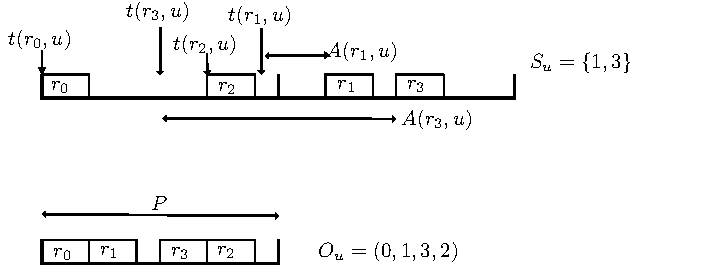
\includegraphics[scale=1]{Chapitre5/normalizedassignment}
\caption{A compact representation of an assignment in which $O_u = (0,1,3,2)$ and $S_u = \{1,3\}$ }
\label{fig:normalizedassignment}
\end{figure}


Remark that for $CR(A)$ to be defined, we need that, on each contention point, at least one datagram is not buffered. We call such an assignment a \textbf{canonical assignment}. It turns out that any assignment $A$ can be made canonical without increasing $TR(A)$, hence we can only consider canonical assignments when solving \spall.

\begin{lemma}\label{lemma:canonical_min}
Let $A$ be a valid assignment, then there is a valid canonical assignment $A'$ such that $A' \preceq A$.
\end{lemma}
\begin{proof}
Consider a vertex $u$ of contention depth $1$, such that for all $r \in \mathcal{R}_u$, $A(r,u) > 0$. Let us define $m$ as the minimum of these values, we define $A'(r,u) = A(r,u) - m$. Assignment $A'$ has no collision on $u$, since all departure times have been shifted by the same value and $A$ has no collision. Moreover, if $v$ is the vertex after $u$ in a route $r$, we define  $A'(r,v) = A(r,v) + m$. Hence, all departure times for vertices of contention depths larger than one are the same in $A$ and $A'$, which implies that there are no collisions in these vertices. We have proven that $A'$ is still valid. Since all departure times of $A'$ are less or equal to those induced by $A$, we have $A' \preceq A$. Moreover, if $r_0$ is the route with $A(r_0,u) = m$, then $A'(r_0,u) = 0$. 

We apply this transformation by increasing contention depth. Since, the transformation applied at some contention depth do not change $A'$ for smaller contention depths, a trivial induction proves that $A'$ is valid, canonical and that $A' \preceq A$.
\end{proof}


\subsection{From a Compact Assignment to its Realization}\label{sec:real}


We now explain how to transform a compact representation into a canonical assignment.
Moreover, we show that the obtained assignment is the smallest among all assignments of same representation. We first explain how to do the transformation on a routed network with a single contention point $u$.

Recall that the datagram of a route $r$ is available at time $t(r,u)$ in the vertex $u$.
Let us consider a compact assignment $CA$, which maps $u$ to the pair $(O_u,S_u)$.
The assignment $Real(CA)$ is built inductively from $CA$, it is called the realization of $CA$. 
If the construction of $Real(CA)$ fails, then $Real(CA)$ is undefined and we say that $CA$ is not realizable. In the next paragraph, we build an assignment $A$ by setting the buffering time of the routes in the order
 $(O_u)$. If the construction suceeds, we set $Real(CA) = A$ 

Let say that the order $O_u$ is $(r_0, \dots, r_l)$. We fix $A(r_0,u)$ to zero, that is the first
datagram in the period has no buffering time. Then, in each period beginning by the first datagram, the datagrams will be in order $O_u$. When the first datagram of the period is chosen, we use it to define normalized arrival times and normalized sending times.
Assume that $A(r_i,u)$ have been set for $i \leq l$, let us explain how to 
set $A(r_{i+1},u)$. If $r_{i+1} \notin S_u$, then $A(r_{i+1},u)$ is chosen so that $ns(r_1,r_{i+1},u)$ is the maximum of $ns(r_1,r_i,u) + \tau$ and $nt(r_1,r_{i+1},u)$. If $ns(r_1,r_{i+1},u) > P - \tau$, then $CA$ is not realizable. If $r_{i+1} \in S_u$, then $A(r_{i+1},u)$ is chosen so that $ns(r_1, r_{i+1},u) = ns(r_1,r_i,u) + \tau$. In both cases, if $ns(r_1, r_{i+1},u) \geq nt(r_1,r_{i+1},u)$, then $CA$ is not realizable (the sending time is in the wrong period with regard to $S_u$). 

Figure~\ref{fig:compacttoassignment} shows how an assignment $Real(CA)$ is built from a compact assignment $CA$ on a single contention point $u$. We have $O_u = (2,1,0,3)$ and $S_u = \{1\}$. First, the datagram $2$ is fixed, that is, $A(r_2,u)=0$. Then, since $r_1 \in S_u$, we set $A(r_1,u)$ such that $ ns(r_2,r_1,u) = ns(r_2,r_2,u) + \tau$. 
Finally, since $r_0$ and $r_3 \notin S_u$, we set $A(r_0,u)$ and $A(r_3,u)$ such that $ns(r_2,r_0,u) = nt(r_2,r_0,u)$ and  $ns(r_2,r_3,u) = ns(r_2,r_0,u) + \tau$.
\begin{figure}[!h]
	\centering
	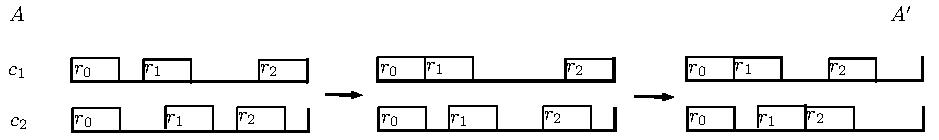
\includegraphics[scale=1]{Chapitre5/compacttoassignment}
\caption{Inductive construction of $Real((2,1,0,3),\{1\})$ from $CA$ on a single contention point $u$. }
\label{fig:compacttoassignment} 
\end{figure}

The function $Real$ can easily be generalized to any routed network. Indeed, one can first consider all vertices of contention depth $1$, the routes going through them form disjoint sets. Hence, we can define $Real$ independently on each vertex of contention depth $1$. 
Then using the buffering computed for these vertices, one can compute the arrival time of each route in vertices of contention depth $2$ and compute $Real$ for these vertices in the exact same way, and so on for all contention depths. In the following lemmas and theorems, we always consider a single contention point, since it is trivial to extend any property for one contention point to the whole routed network as we just explained. 

\begin{lemma}\label{lemma:canonical}
The assignment $Real(CA)$ can be computed in time $O(nd)$, where $d$ is the contention
depth of the network. If $CA$ is realizable, then $Real(CA)$ is a valid canonical assignment.
\end{lemma}
\begin{proof}
In the inductive construction of $Real(CA)$, only a constant number of comparisons and additions are needed to compute the 
buffer time of a route from the previous one. Hence, the time spent in a vertex $u$ is linear in $|\mathcal{R}_u|$. 
A route can go through only one vertex of a given contention depth, hence the time spent computing buffers for all vertices
of a contention depth is in $O(n)$ and for the whole graph it is in $O(nd)$.

To prove that there is no collision between pair of routes for a given assignment, it is enough to 
prove it for any interval of time of size $P$. Hence, it is enough to consider the normalized sending time and to verify
they do not induce a collision. By construction,  $ns(r_1,r_{i+1},u)$ is always larger than $ns(r_1,r_{i},u) + \tau$ and less 
than $P - \tau$, which proves the absence of collision. Finally, $Real(CA)$ is canonical, since by definition $Real(CA)(r_1,u) = 0$, where $r_1$ is the first route in $O_u$.
\end{proof}

We can define the following equivalence relation over canonical assignments: $A$ and $B$ are equivalent if and only if $CR(A) = CR(B)$.
We say that a compact assignment $CA = (O_u,S_u)_{u \in V(G)}$ is \emph{canonical} if it is a realizable compact assignment, $CR(Real(CA)) = (O'_u,S'_u)_{u \in V(G)}$ and if for all vertices $u$, the first routes of $O_u$ and $O'_u$ coincide. This notion of canonicity is defined so that the function $CR$ always sends a canonical assignment on a canonical compact assignment. It is just restrictive enough (by fixing the first element in each order), that the function $CR$ is the inverse of $Real$ over canonical compact assignments. It implies that $Real(CA)$ can be chosen as the representative of the equivalence class of the assignments having $CA$ as a representation.

In fact, as implied by the following Lemma, we can be more precise on $Real(CA)$: it is minimal for $\prec$ in its equivalence class.

\begin{lemma}\label{lemma:prec}
Let $A$ be a valid assignment, then $Real(CR(A)) \preceq A$.
\end{lemma}
\begin{proof}
Given a vertex $u$ and a route $r \in \mathcal{R}_u$, we prove by induction that $Real(CR(A))(r,u) \leq A(r,u)$.
Let $(O_u,S_u)$ be the pair associated to $u$ by $CR(A)$, with $O_u = (r_1,\dots,r_l)$. By definition of $CR$, $r_1$ the first route in $O_u$, is such that $A(r_1,u) = 0$. By definition of $Real$, we have that  $Real(CR(A))(r_1,u) = 0 = A(r_1,u)$.
Now assume that $Real(CR(A))(r_i,u) \leq A(r_i,u)$ for some $i$. 

First, consider the case $r_{i+1} \notin S_u$. By definition of $CR$, $ns(r_1,r_{i+1},u)$ must be larger than 
$ns(r_1,r_{i},u)+ \tau$ and because $r_{i+1} \notin S_u$ it must also be larger than $rs(r_1,r_{i+1},u)$. 
Since $Real(CR(A))(r_{i+1},u)$ is the minimum value so that both constraints are true for $Real(CR(A))$, using
the induction hypothesis, we have $Real(CR(A))(r_{i+1},u) \leq A(r_{i+1},u)$. The case $r_{i+1} \in S_u$ is similar and left to the reader.
\end{proof}


\section{Greedy Algorithms}
 
 In the next section, we propose several local search algorithms to explore the compact assignments in order to find a compact assignment $CA$ with the smallest possible $TR(Real(CA))$. A realizable compact assignment is needed to initialize these local search algorithms. To find such initial compact assignment, we propose in this section three greedy algorithms which try to build canonical valid assigments, which can be turned into a compact representation by the $CR$ function.

\subsection{Greedy Deadline}

We first present a simple algorithm, which is the natural approach in a context witout \emph{periodicity}.
The contention points are sorted by contention depth, and the contention depths are dealt with in ascending order. The assignment, on contention points of the same contention depth, is computed independently. The \greedydeadline algorithm consists in selecting among the routes of arrival time less than the current time the one with the longest transmission time. If no route are available at the current time, select the one with the smallest arrival time.

More precisely, \greedydeadline works as follow. For a vertex $u$, select the route $r$ such that the arrival time $t(r,u)$ is minimal and fix $A(r,u) = 0$. Assume that some datagrams have now been scheduled, the last one on the route $r$ at time $s(r,u)$, we explain here how to schedule the next route.  If there are several routes $r'$ for which $t(r',u) < s(r,u) + \tau $, we need to select one of those. For each $r'$ with the previous property, we compute the value $\lambda(r,u) - t(r',u)$ and select the one which minimizes this value. Then, the selected datagram $r'$ is sent with a delay $A(r',u) = t(r,u) + \tau - t(r',u)$. If no route satifies $t(r',u) < s(r,u) + \tau$, the route with the lowest $t(r,u)$ is sent without delay ($A(r',u) = 0$). 
Due to the periodicity, once the route $r'$ has been selected and $s(r',u)$ computed, it is possible that there is a collision. If so, $s(r',u)$ is increased to the first time such that there is no collision. If there is no such time, the algorithm fails.


%\begin{algorithm}[H]
%	\caption{\greedydeadline}
%	\begin{algorithmic}
%	\REQUIRE $(G,{\cal R})$, $P$, $\tau$
%	\ENSURE An assignment $A(G,{\cal R})$, or FAILS
%	\STATE $budget[|{\cal R}|]$ integer table.
%	\FORALL{route $r$ in ${\cal R}$}
%      \STATE  $budget[r] \leftarrow \lambda(u,r) - t(r,u)$
%	\ENDFOR
%	\STATE Let $first$ be the route such that $t(first,u)$ is minimal
%	\STATE $A(first,u) \leftarrow 0$
%	\STATE $offset \leftarrow t(first,u)+\tau$
%	\STATE ${\cal R} \leftarrow {\cal R}\setminus \{first\}$
%    \WHILE{ ${\cal R} \neq \emptyset$}
%    \IF {$\exists i \in{\cal R}, t(i,u) \leq offset$}
%   \STATE Choose $i$ with the lowest $budget[i]$
%    \STATE $A(i,u) \leftarrow offset - t(i,u)$
%    \STATE $offset \leftarrow offset + \tau$
%    \ELSE
%     \STATE Choose $i \in {\cal R}$ with the lowest $t(i,u)$
%     \STATE $A(i,u) \leftarrow 0$
%     \STATE $offset \leftarrow t(i,u) + \tau$
%    \ENDIF
%    \IF{$A$ is not valid}
%    \IF{ $add\_delay \leftarrow FIRST\_VALID(A,P,i)$}
%    \STATE $A(i,u) \leftarrow A(i,u) + add\_delay$
%    \ELSE
%   \STATE Return FAIL
%    \ENDIF
%    \ENDIF
%    
%    \ENDWHILE
%    \STATE Return SUCCESS
%	\end{algorithmic}
%	\end{algorithm}

   \begin{figure} 
	\centering
	\includegraphics[scale=0.8]{Chapitre5/examplegreedyfail}
\caption{An instance for which \greedydeadline fails to build an assignment}
\label{fig:examplegreedyfail}   
\end{figure}



\subsection{Greedy Normalized}

We present here a variant of \greedydeadline: select as first datagram the one with minimal $t(r,u)$, then select the datagrams by lowest normalized arrival times instead of arrival times. Let us call this algorithm
\greedynormalized. In practice, it performs better than \greedydeadline.

Both \greedydeadline and \greedynormalized may fail to find a valid assignment for some routed networks, for which there exist a valid assignment. The way we select departure times for the routes can create unused interval of time of size less than $\tau$. These intervals are not usable to schedule datagram of size $\tau$. If too much time is wasted in this way, the algorithms will fail, while there is always a valid assignment when the load is less or equal to $1$. Since each datagram forbids at most $2\tau -1$ tics in the period to the other datagrams, by a pigeonhole argument, all routes can be scheduled by greedy algorithms considering all departure times, when the load is less than $0.5$ (see Chapters~\ref{chap:PAZL} for similar arguments).



\subsection{Greedy Packed}


A compact assignment is needed to initialize the local search algorithms presented in the next section. Hence, we propose the \greedypacked algorithm that is guaranteed to find an assignment, even if the transmission time may be worse on average than what is found by the two previous greedy algorithms.
The contention points are still managed level by level. For a vertex $u$, we explain how to build the pair $(O_u,S_u)$. First, the route with the lowest arrival time is selected, say $r_0$ and we say that $0$ is the first element of $O_u$ and $0 \notin S_u$. From now on, $r_0$ is used to define the normalized arrival times of the other routes. Assume that $(r_0,\dots,r_i)$, the first $i$ routes of $O_u$ are chosen, let us explain how to choose the $i+1$th route. If there are routes with a normalized arrival time lower or equal to $ns(r_0,r_i,u)+\tau$, the route $r$ with the smallest value of $\lambda(r,u) - t(r,u)$ is chosen (as in \greedynormalized). If no route satisfy this property, then let $r$ be the route which minimizes $\lambda(r,u) - t(r,u) - nt(r_0,r,u)$, choose it, and $S_u = S_u \cup \{r\}$. In other words, select the route with the smallest transmission time if scheduled without creating gap in the period.


\subsection{Random generation of routed network}
\label{sec:generationrouted}
This chapter presents several algorithms that each have several variants or parameters to tune. Thus, each section or subsection describing a new algorithm also provide some experimental results. We describe here how the instances are generated for every experiment of the chapter until Section~\ref{sec:evalperfspall} that present more general performance evaluations.

First, remark that, contrary to our choice for star routed networks, we consider that the physical length of the links into the datacenter are the same for all routes. Indeed, several BBUs are often gathered in one or several datacenters. The length of the links between the entrance of the datacenter and all BBUs may or may not be the same. In the first case, once the messages have been scheduled to go in the datacenter, they go out in the exact same order and thus, even if all routes use the same link in the way back, it is not considerd as a contention point (see figure~\ref{fig:bbuaggreg}), and the routes are symmetrical around the vertex representing the entrance in the BBU. If the length of the links into some datacenter are different, the aggregation node before the datacenter is represented by two contention points. The datagrams may collide in both the entrance and the exit of the datacenter and the routes are symmetrical around the arc between the two contention points.

    \begin{figure}

  \centering
  \includegraphics[scale=0.8]{Chapitre5/bbuaggreg}


\caption{One or several contention points around the BBU according to the lenght of the link}
\label{fig:bbuaggreg}
\end{figure}

We propose several experiments to assess the practical performance (in speed and quality) of the poposed algorithms. We present here the instances on which we test our algorithms, which are derived from our application to Cloud-RAN. We consider networks of contention depth three, as illustrated in Figure~\ref{fig:randomnetworks}, in which each dotted arc represents the arcs of two routes. 



\begin{figure}
\begin{center}
\scalebox{0.4}{

\begin{tikzpicture}
  \SetGraphUnit{5}
    \tikzset{
  EdgeStyle/.append style = {->} }
   \tikzstyle{VertexStyle}=[shape = circle, draw, minimum size = 30pt]
 

  \node (s8) at (0,10.5) {
\includegraphics[width = 1cm]{rrh.png}};
  \node (s7) at (0,9) {
\includegraphics[width = 1cm]{rrh.png}};
  \node (s6) at (0,7.5) {
\includegraphics[width = 1cm]{rrh.png}};
  \node (s5) at (0,6) {
\includegraphics[width = 1cm]{rrh.png}};
  \node (s4) at (0,4.5) {
\includegraphics[width = 1cm]{rrh.png}};
  \node (s3) at (0,3) {
\includegraphics[width = 1cm]{rrh.png}};
  \node (s2) at (0,1.5) {
\includegraphics[width = 1cm]{rrh.png}};
  \node (s1) at (0,0) {
\includegraphics[width = 1cm]{rrh.png}};
  
   \node (b2) at (10,7.25) {
\includegraphics[width = 1cm]{bbu.png}};
   \node (b1) at (10,2.25) {
\includegraphics[width = 1cm]{bbu.png}};

   \node (t6) at (8,7.25) {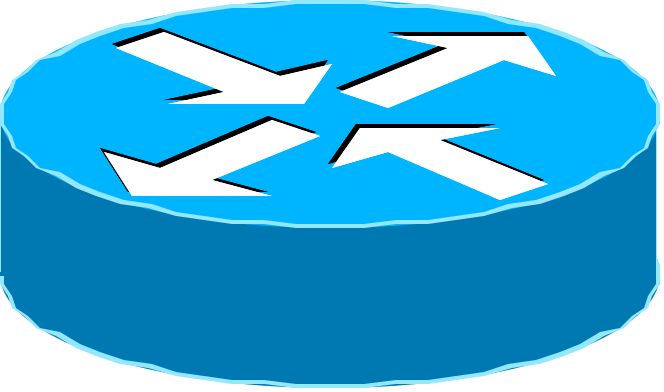
\includegraphics[width = 1cm]{switch.png}};
   \node (t5) at (8,2.25) {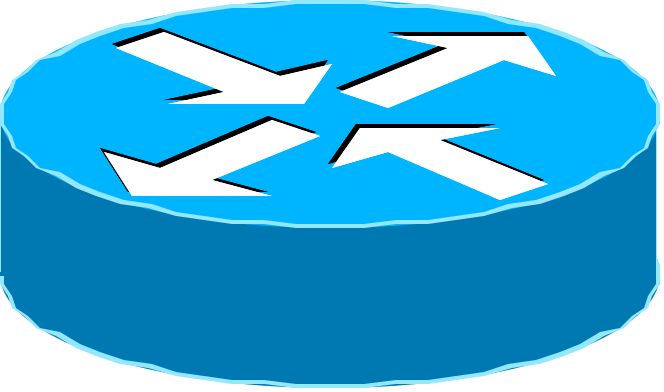
\includegraphics[width = 1cm]{switch.png}};
   \node (t4) at (4,9.75) {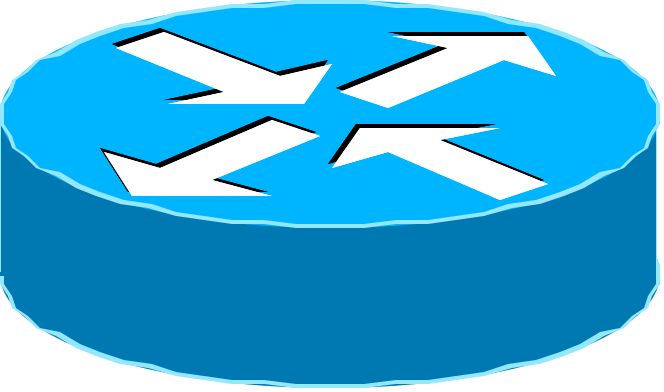
\includegraphics[width = 1cm]{switch.png}};
   \node (t3) at (4,6.75) {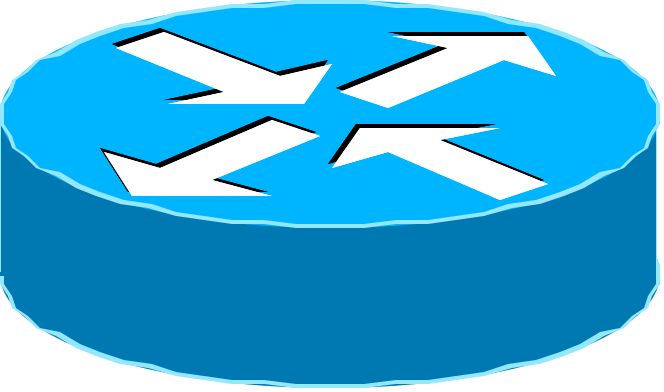
\includegraphics[width = 1cm]{switch.png}};
   \node (t2) at (4,3.75) {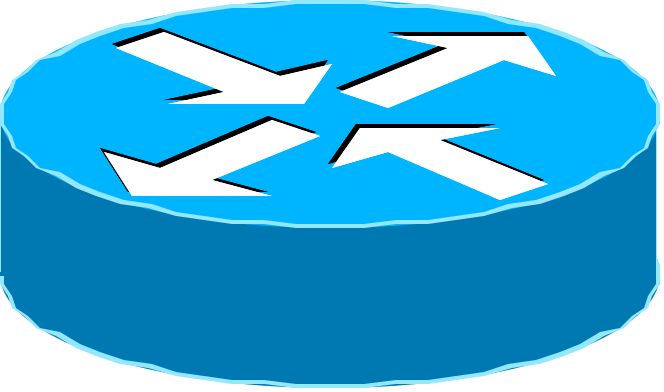
\includegraphics[width = 1cm]{switch.png}};
   \node (t1) at (4,0.75) {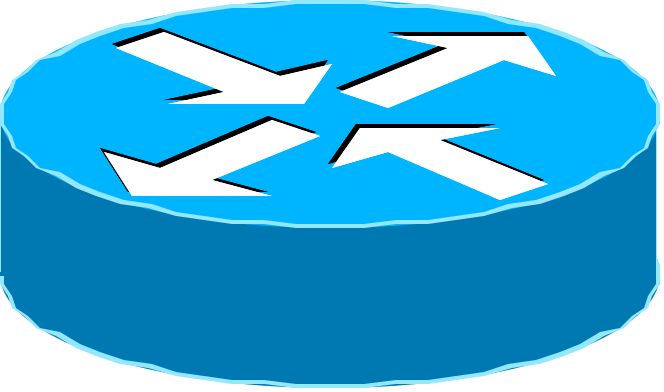
\includegraphics[width = 1cm]{switch.png}};

\path (s1) edge [<->,blue]  (t1);
\path (s2) edge [<->,green]  (t1);
\path (s3) edge [<->,red]  (t2);
\path (s4) edge [<->,orange]  (t2);
\path (s5) edge [<->,brown]  (t3);
\path (s6) edge [<->,purple]  (t3);
\path (s7) edge [<->,pink]  (t4);
\path (s8) edge [<->]  (t4);

\path (t1) edge [<->,blue]  (t5);
\path (t1) edge [<->,green]  (t6);
\path (t2) edge [<->,red]  (t5);
\path (t2) edge [<->,orange]  (t6);
\path (t3) edge [<->,brown]  (t5);
\path (t3) edge [<->,purple]  (t6);
\path (t4) edge [<->,pink]  (t5);
\path (t4) edge [<->]  (t6);

\path (t6) edge [<->,thick]  (b2);
\path (t5) edge [<->,thick]  (b1);


\node (k8) at (30,10.5) {$t_8$};
\node (k7) at (30,9) {$t_7$};
\node (k6) at (30,7.5) {$t_6$};
\node (k5) at (30,6) {$t_5$};
\node (k4) at (30,4.5) {$t_4$};
\node (k3) at (30,3) {$t_3$};
\node (k2) at (30,1.5) {$t_2$};
\node (k1) at (30,0) {$t_1$};

  \node (s8) at (14,10.5) {$s_8$};
  \node (s7) at (14,9) {$s_7$};
  \node (s6) at (14,7.5) {$s_6$};
  \node (s5) at (14,6) {$s_5$};
  \node (s4) at (14,4.5) {$s_4$};
  \node (s3) at (14,3) {$s_3$};
  \node (s2) at (14,1.5) {$s_2$};
  \node (s1) at (14,0) {$s_1$};


  
  \node (t10) at (26,9.75) {$c_{10}$};
   \node (t9) at (26,6.75) {$c_9$};
   \node (t8) at (26,3.75) {$c_8$};
   \node (t7) at (26,0.75) {$c_7$};
   \node (t6) at (22,7.25) {$c_6$};
   \node (t5) at (22,2.25) {$c_5$};
   \node (t4) at (18,9.75) {$c_4$};
   \node (t3) at (18,6.75) {$c_3$};
   \node (t2) at (18,3.75) {$c_2$};
   \node (t1) at (18,0.75) {$c_1$};

\path (s1) edge [->,blue]  (t1);
\path (s2) edge [->,green]  (t1);
\path (s3) edge [->,red]  (t2);
\path (s4) edge [->,orange]  (t2);
\path (s5) edge [->,brown]  (t3);
\path (s6) edge [->,purple]  (t3);
\path (s7) edge [->,pink]  (t4);
\path (s8) edge [->]  (t4);

\path (t1) edge [->,blue]  (t5);
\path (t1) edge [->,green]  (t6);
\path (t2) edge [->,red]  (t5);
\path (t2) edge [->,orange]  (t6);
\path (t3) edge [->,brown]  (t5);
\path (t3) edge [->,purple]  (t6);
\path (t4) edge [->,pink]  (t5);
\path (t4) edge [->]  (t6);

\path (k1) edge [->,blue]  (t7);
\path (k2) edge [->,green]  (t7);
\path (k3) edge [->,red]  (t8);
\path (k4) edge [->,orange]  (t8);
\path (k5) edge [->,brown]  (t9);
\path (k6) edge [->,purple]  (t9);
\path (k7) edge [->,pink]  (t10);
\path (k8) edge [->]  (t10);

\path (t7) edge [->,blue]  (t5);
\path (t7) edge [->,green]  (t6);
\path (t8) edge [->,red]  (t5);
\path (t8) edge [->,orange]  (t6);
\path (t9) edge [->,brown]  (t5);
\path (t9) edge [->,purple]  (t6);
\path (t10) edge [->,pink]  (t5);
\path (t10) edge [->]  (t6);




\end{tikzpicture}
}



%\end{minipage}

             \caption{Left, a physical fronthaul network and right, the routed network modeling a round trip in the fronthaul network. Each route is represented by the arcs of the same color.}

           \label{fig:randomnetworks}
            \end{center}
           \end{figure}
%
%   \begin{figure} 
%	\centering
	%\includegraphics[scale=0.8]{Chapitre5/networksrandom}
%
%\caption{Shape of the randomly generated routed networks: $4$ vertices of contention depth $1$, each with two routes going through, which go to the two different data centers in contention depth $2$}
%\label{fig:randomnetworks}
%\end{figure}

To generate random routed networks, several parameters must be chosen: The load of the network, the number of routes, the distribution of the length of the arcs, and the topology of the routed network. We would like to understand the impact of those parameters, in terms of computation time and quality, for each of the algorithms studied. In order to reduce the number of experiences presented here, we fix the topology of the routed network to the one shown in Figure~\ref{fig:randomnetworks}. The difference between the performances of the presented algorithms are not significantly impacted if we change the number of contention points. 

 
 The impact of the load on the quality of the results has been investigated: When the load is increased, the relative quality of solutions found by the local search algorithms does not changes significantly. Hence, we choose to fix the load to $0.8$, which is an already high load. This means that $P = \frac{\tau \times n}{0.8}$, whith $n$ the maximal number of routes over a contention point. The size of the C-RAN traffic depends of the service requirement~\cite{mobile2011c}. Here, we fix $\tau = 2500$ tics.
  
In a C-RAN context, the number of route is low. In the network we study, there is $n=8$ routes on the graph. This kind of graphs with few routes allows us to use the Branch and Bound algorithm to find the ptimal solution for evaluating the performances of the other algorithms. We study the impact of the number of routes in the graph in Section~\ref{sec:evalperfspall}. The length of the arcs is drawn uniformly between $0$ and $P$. This choice makes the periodicity of our problem impactful, and does not allow  us to reuse algorithms from a non periodic setting.

We also recall the notion of \textbf{margin} of a route $r$, which is equal to $D - \lambda(r)$, that is, the difference between the deadline and the physical delay of the route. In other words, this represent the time allowed for logical delays, that are set by the assignments. The margin of the routed network is the minimum of the margins of the routes
and we will often express the performance of our algorithms as the value of the margin for which they solve \spall.



\subsection{Success Rate and Performance of the Greedy Algorithms}


We want to compare the succes rate and the performance of the different algorithms presented in this section.
First, we consider the impact of the load of the network on the succes rate of the three greedy algorithms. We have explained that all greedy algorithms succeed when the load is less than $0.5$ and that \greedypacked always succeeds.
Figure~\ref{tab:success} shows the success rate of \greedydeadline and \greedynormalized on $1000$ random instances for loads from $0.7$ to $1$. %The graph are gererated as explained in section~\ref{subsection:CRANGRAPH}.
 \greedydeadline fails less than \greedynormalized on highly loaded networks, while \greedynormalized seems more robust on loads between $0.8$ and $0.9$. 
\begin{center}
\begin{figure}
\centering
\begin{tabular}{ |c|c|c|c|c| }
\hline
    \backslashbox{Sucess}{Load} & $0.7$ & $0.8$& $0.9$& $1$ \\
    \hline
    \greedydeadline & $99.5\%$ & $92.4\%$& $43.4\%$& $15.7\%$ \\
 
    \greedynormalized & $99.3\%$ & $93.2\%$& $51.2\%$& $0\%$ \\
   
  %  GP & $100\%$ & $100\%$& $100\%$& $100\%$ \\
    \hline
  
 \end{tabular}
 \caption{Success rate of the greedy algorithms for different loads}
 \label{tab:success}
 \end{figure}
 \end{center}

 We now want to compare the quality of the solution found by these algorithms.  Figure~\ref{fig:90load} shows the margin needed by the assignments given by the algorithms, when there is one. As expected, \greedypacked, that trades margin for success rate, performs worse than \greedydeadline and \greedynormalized when they are able to find an assignment. \greedynormalized performs better than \greedydeadline when it finds an assignment.  On vertices with high load, the three algorithms almost always find the same assignment (or fail). On vertices of small load, the constraint of packing the datagram imposed by \greedydeadline worsen the latency.

We propose an improved version of \greedydeadline and \greedynormalized that always find a solution. For each contention point, we first try \greedydeadline (or \greedynormalized), and if the algorithm fails, we apply \greedypacked. Let us call \hybridgreedydeadline and \hybridgreedynormalized those two algorithms. Figure~\ref{fig:greedysuccess} shows the performances of \hybridgreedydeadline, \hybridgreedynormalized, and \greedypacked on $1000$ routed networks. Here, the load is of $0.9$ to emphasize the difference between algorithms.

 	\begin{figure}
	\centering
	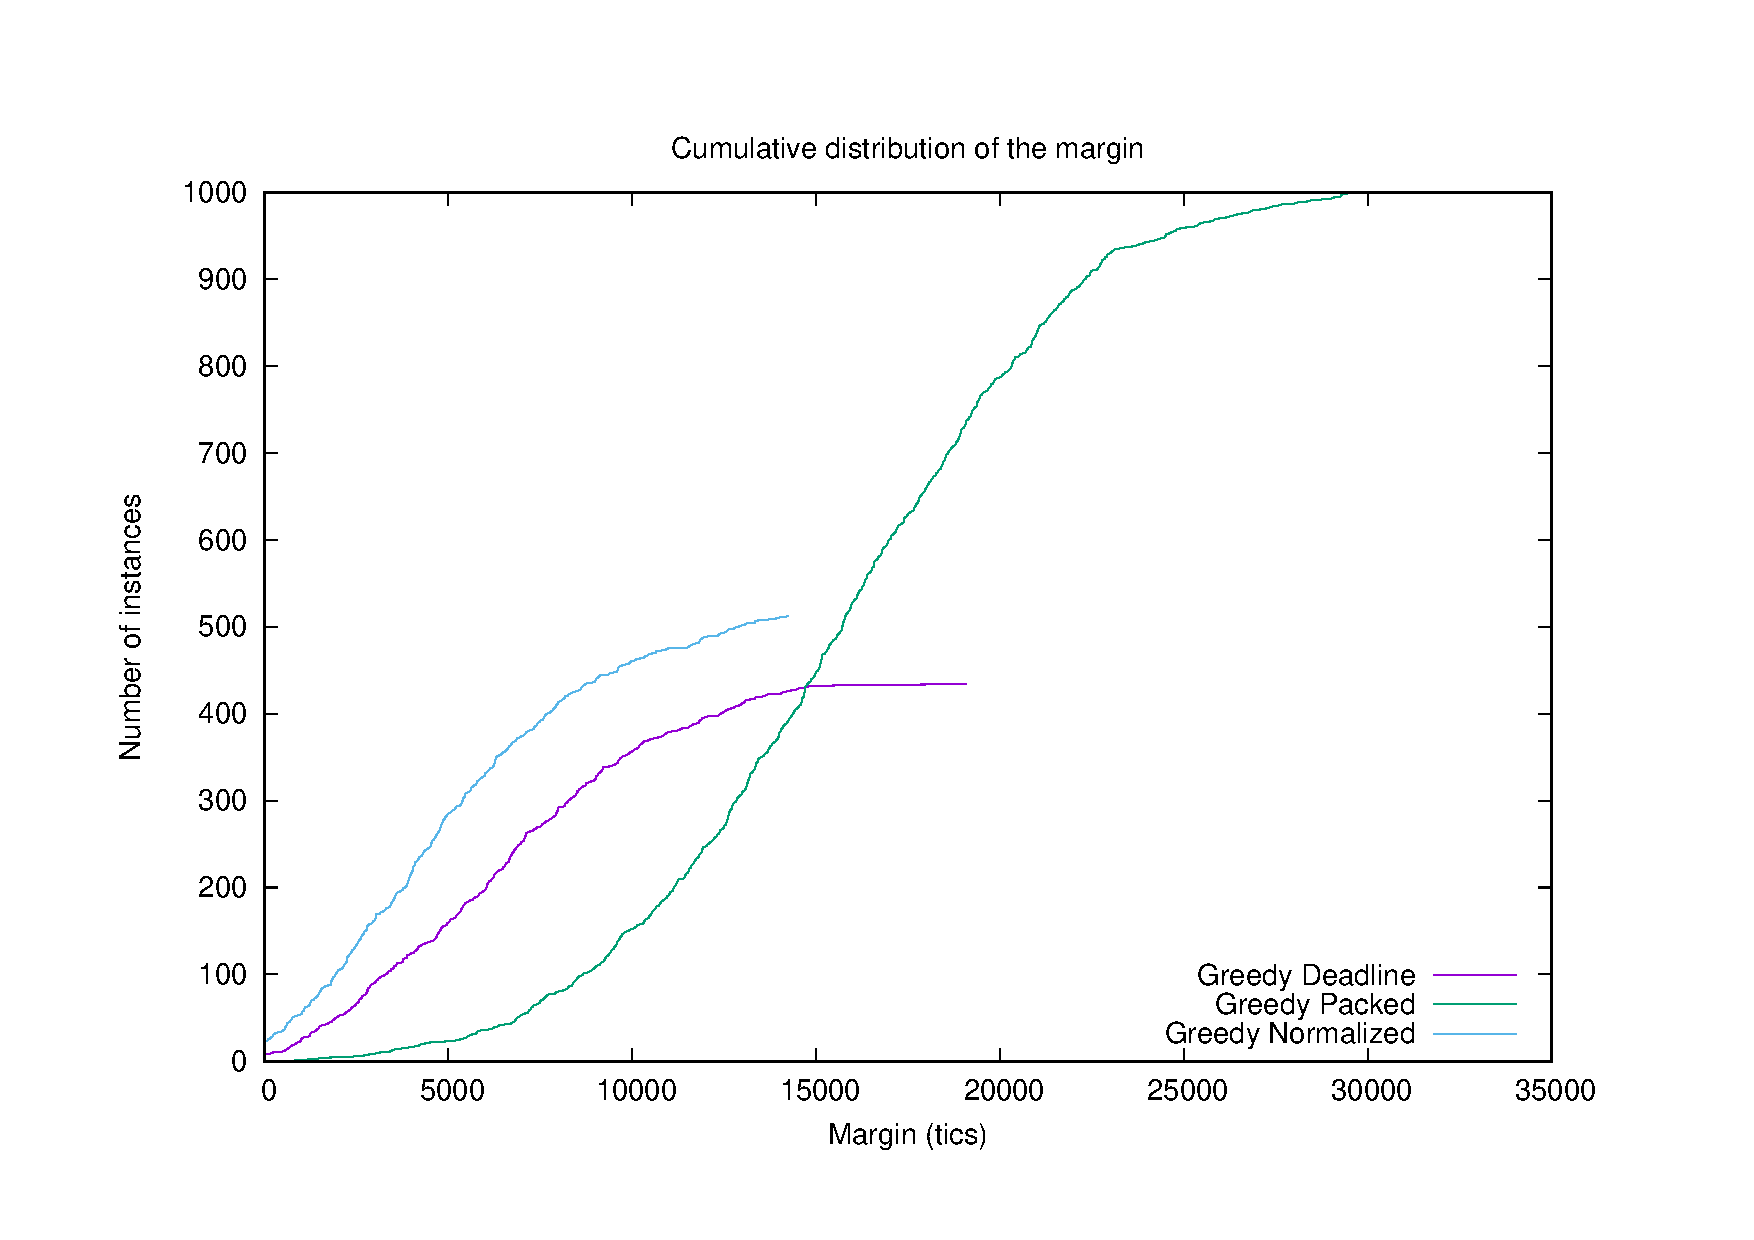
\includegraphics[scale=0.5]{Chapitre5/90load}
\caption{Performance of \greedydeadline, \greedynormalized and \greedypacked. Curves of \greedydeadline and \greedynormalized are incompelte because only the instances for which a solution is found are represented here.}
\label{fig:90load}
\end{figure}


\begin{figure}
	\centering
	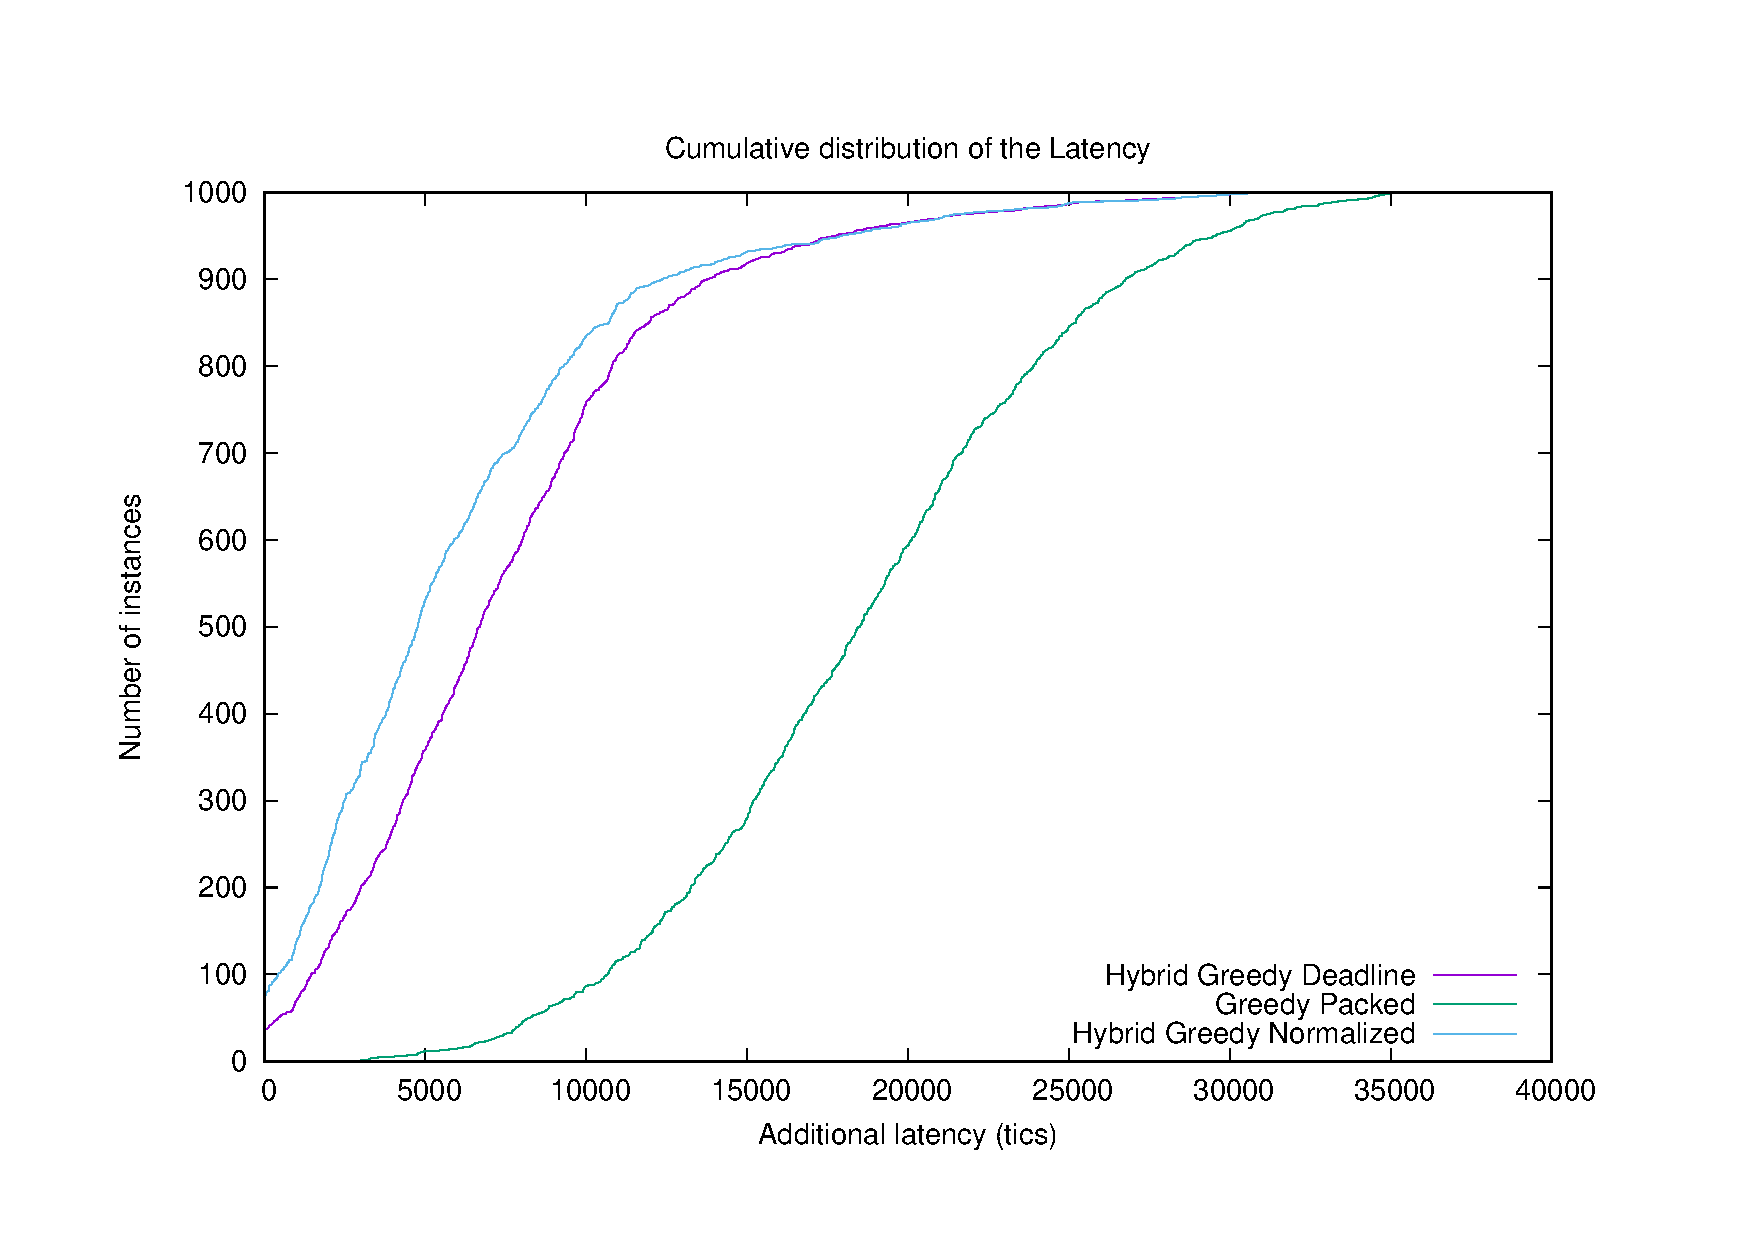
\includegraphics[scale=0.5]{Chapitre5/greedysuccess}
\caption{Performance of the updated greedy algorithms that always gives an assignment} 
\label{fig:greedysuccess}
\end{figure}

Algorithm \hybridgreedynormalized seems much better than the other two. Hence, in the rest of the paper \hybridgreedynormalized will serve as a baseline of assignment quality since it can be obtained in very short time. It will also serve to initialize 
local search algorithms with a first assignment of sufficient quality.

\section{Local Search Heuristics}

The number of compact assignments $CA$ grows extremely quickly with $n$. Hence, to find one which minimizes $TR(Real(CA))$, we propose several classical local search algorithm: Hill Climbing, Tabu Search and Simulated Annealing. These methods work as long as a relevant notion of neighborhood of a solution is proposed. The neighborhood relation must satisfy two properties: it must be quick to compute (hence not too large) and the implicit graph of solutions defined
by the neighborhood relation should be connected. We now propose a simple neighborhood relation over compact assignments.

Let $u$ be a contention point of a network, and let $CA$ be a compact assignment for this network, 
 which associates the pair $(O_u,S_u)$ to $u$. Let $O_u = (r_1,\dots,r_l)$ and let $\triangle$ denotes the symmetric difference.   Let $r_i \in \mathcal{R}_u$, the \emph{$r_i$-neighborhood} of $(O_u,S_u)$ is the set of pairs $(O,S)$ such that:
 
 \begin{enumerate} 
 \item $O = O_u$ and $S_u = S$ or $S \triangle \{r_i\}$  
 \item $O = (r_1,\dots,r_{i-2},r_{i},r_{i-1},\dots,r_{l})$ and $S_u = S$ or $S \triangle \{r_i\}$ or  $S \triangle \{r_{i-1}\}$ or $S \triangle \{r_i,r_{i-1}\}$ 
 \end{enumerate}

Informally, a compact assignment is in the $r$-neighborhood of another one if it can be obtained by 
moving down $r$ once (or not changing it) in the order and adding or removing $r$ and the previous route from the set. 
Remark that the $r$-neighborhood of any pair $(O_u,S_u)$ has at most $6$ members (it can be $4$ when the route $r$ is in first position and cannot be exchanged with the previous one). Figure~\ref{fig:partialtreeneigh} represent the $r$-neighborhood of a pair $(O_u,S_u)$.

The \emph{$r$-neighborhood} of a compact assignment $CA$ is the set of all compact assignments $CA'=(O'_u,S'_u)_{u \in V(G)}$, such that  $(O'_u,S'_u)$ is in the $r$-neighborhood of $(O_u,S_u)$. Finally, the \emph{neighborhood} of a compact assignment $CA$ is the union for all $r \in {\cal R}$ of the $r$-neighborhoods of $CA$.  

 Let us denote by $k_1,\ldots,k_n$ the number of contention points on the $n$ routes of 
 a routed network. Then, a compact assignment has at most $\sum_{i=1}^n 6^{k_i}$ neighbors. Since the networks we consider are of bounded contention depth ($2$ or $3$ in practice), the size of a neighborhood is linear in the number of routes.  We further restrict the notion of neighborhood to realizable compact assignments. Indeed, the unrealizable compact assignments do not yield a real assignment, their transmission time is not defined and we cannot use them in our local search algorithms. We call the graph defined by the neighborhood relation over realizable compact assignments of a routed network the {\bf transposition graph} of the routed network. 
  All algorithms presented in this section will do a walk in the transposition graph, trying to find a vertex with optimal
  transmission time. 

\begin{figure}
\begin{center}
\scalebox{0.4}{

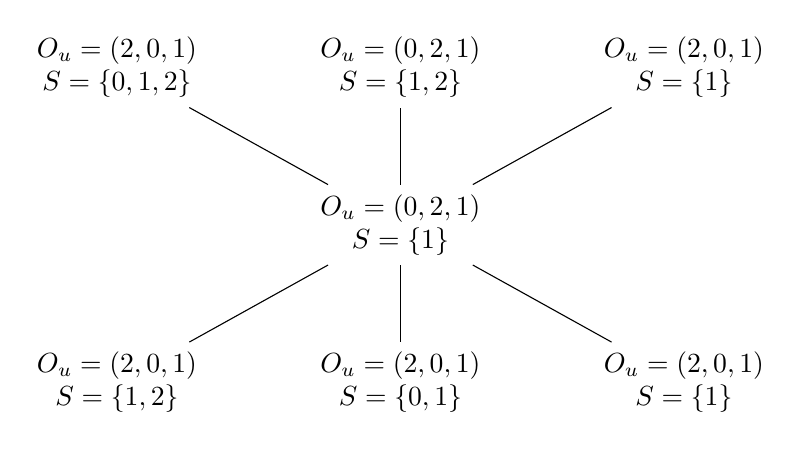
\begin{tikzpicture}
  \SetGraphUnit{5}
    \tikzset{
  EdgeStyle/.append style = {->} }
   \tikzstyle{VertexStyle}=[shape = circle, draw, minimum size = 50pt]
 

  \node[align=center] (p0) at (10,5) {$O_u = (0,2,1)$\\$S = \{1\}$};
  \node[align=center] (p1) at (10,7) {$O_u = (0,2,1)$\\$S = \{1,2\}$};
  \node[align=center] (p2) at (13.6,7) {$O_u = (2,0,1)$\\$S = \{1\}$};
  \node[align=center] (p3) at (13.6,3) {$O_u = (2,0,1)$\\$S = \{1\}$};
  \node[align=center] (p4) at (10,3) {$O_u = (2,0,1)$\\$S = \{0,1\}$};
  \node[align=center] (p5) at (6.4,3) {$O_u = (2,0,1)$\\$S = \{1,2\}$};
  \node[align=center] (p6) at (6.4,7) {$O_u = (2,0,1)$\\$S = \{0,1,2\}$};


 
\path (p0) edge [-] (p1);
\path (p0) edge [-] (p2);
\path (p0) edge [-] (p3);
\path (p0) edge [-] (p4);
\path (p0) edge [-] (p5);
\path (p0) edge [-] (p6);



\end{tikzpicture}
}


 \caption{Neighborhood of a pair $O_u = (0,2,1)$, $S_u = \{1\}$ for one contention point.}

\label{fig:partialtreeneigh}
\end{center}
\end{figure}

\begin{lemma}\label{lemma:path}
There is a path from a realizable compact assignment CA, with $CA(u) = (O_u,S_u)$ to $CA'$, such that 
$CA'$ is equal to $CA$ except on $u$ where it is equal to $(O_u,S_u \cup E)$.  
\end{lemma}
\begin{proof}
The path is by adding elements in $E$ one by one. 
 To prove the existence of the path, it is enough to prove that for  $E = \{v\}$. By definition, $(O_u,S_u \cup{v})$ is in the neighborhood of $(O_u,S_u)$. However, one should also prove that $CA'$ is realizable.
  Since the order in which the buffers are fixed by the algorithm of $Real$ is the same for $(O_u,S_u)$ and $(O_u,S_u \cup{v})$, it is easy to prove by induction that the normalized sending times of $(O_u,S_u \cup{v})$ are less than the normalized sending times of $(O_u,S_u)$. Thus, $CA$ realizable implies $CA'$ realizable. Indeed, 
a compact assignment is realizable if and only if the last normalized sending time is less than $P - \tau$.
\end{proof}



 \begin{theorem}
 The transposition graph of a routed network is connected.
 \end{theorem}
 \begin{proof}
 We prove the result for a routed network with a single contention node $u$, it can be generalized to any routed networks 
 by applying the proof contention node by contention node. Let $(O_u,S_u)$ and $(O'_u,S'_u)$ be two realizable compact assignments, we show there is a path between them. Let $r$ be the first element of 
$O_u$ and let $E = \mathcal{R}_u \setminus \{ r \}$. By Lemma~\ref{lemma:path}, there is a path from 
$(O_u,S_u)$ to $(O_u,E)$. Consider now $O_u''$, the order $O_u'$ whith $r$ placed in first position.
There is a path from $(O_u,E)$ to $(O_u'',E)$. Indeed, any order is realizable, when all elements but the first
are in $E$ because there are no constraints on their normalized sending time. 
Now, let $r'$ be the first element of $O_u'$. By definition, $(O_u',E \triangle \{r,r'\})$ is in the $r'$ neighborhood of $(O_u'',E)$. Moreover, $(O_u',E \triangle \{r,r'\})$ is realizable because $E \triangle \{r,r'\}$ is equal to all routes but the first in $O_u'$. 
Finally, using Lemma~\ref{lemma:path} once again prove there is a path between $(O_u',E \triangle \{r,r'\})$ and $(O'_u,S'_u)$ since $(O'_u,S'_u)$ is realizable and $S'_u \subseteq E \triangle \{r,r'\}$, which proves the theorem.
 \end{proof}




\subsection{Hill Climbing}\label{sec:hillclimb}

The most simple local search heuristic is Hill Climbing. This algorithm starts from a compact assignment $CA$, explore the entire neighborhood of $CA$, and selects the realizable compact assignment $CA'$ of minimal transmission time. Then, we set $CA = CA'$ and repeat this step until there are no $CA'$ such that $TR(CA') < TR(CA)$. Then, the algorithm stops and returns $Real(CA)$ which is a local minimum. 

The quality of Hill Climbing depends on the the initial compact assignment. A first choice is to consider the compact representation $CR(A)$ of the assignment $A$ given by \hybridgreedynormalized (\hgn). We can also choose a random compact assignment. Since a compact assignment does not always give a valid assignment nor a good one, we should draw many random compact assignments and return the best assignment found by Hill Climbing using these initial solutions.

Figure~\ref{fig:descente07} shows the difference between initalizing Hill Climbing with \hybridgreedynormalized, or with one or several random compact assignments. Those results are computed from $1000$ random instances, with load of $0.8$.
\begin{figure}[h] 
	\centering
	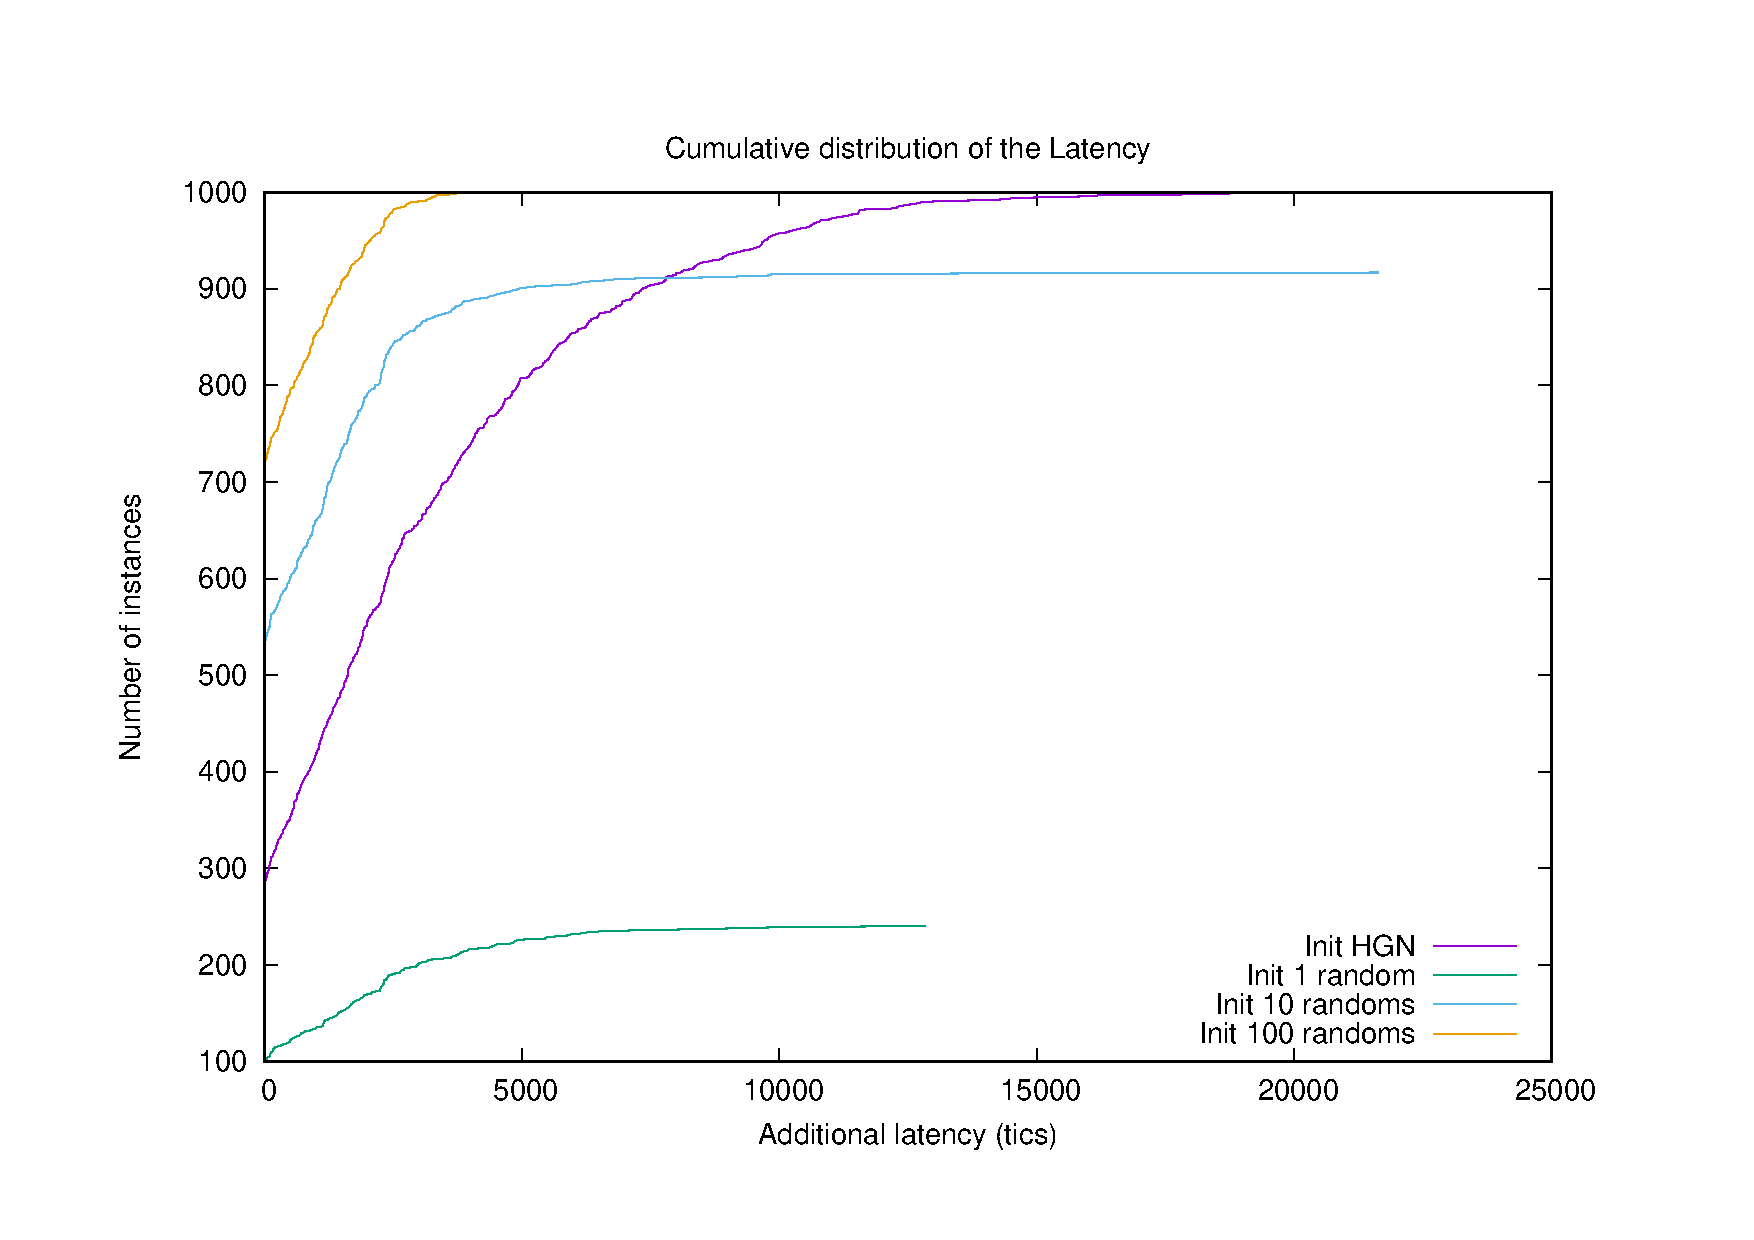
\includegraphics[scale=0.3]{Chapitre5/descente07}
\caption{ Margin needed to find a solution for Hill Climbing, intialized with \hgn, $1$, $10$ or $100$ random compact assignments.}
\label{fig:descente07}
\end{figure}

Initializing Hill Climbing with $100$ random compact assignments seems to give better results. However, 
choosing $100$ random compact assignments can still fail to produce one valid assignment. We investigate this issue
in experiments presented in Figures~\ref{tab:descenteload} and \ref{tab:descentenbroutes}. We represent the probability of drawing at least one compact assignment that gives a valid assignment, when drawing $1$, $10$ or $100$ random compact assignments. In Figure~\ref{tab:descenteload}, we fix the number of routes to $8$, and we change the load from $0.8$ to $1$. In Figure~\ref{tab:descentenbroutes}, we fix the load to $0.8$ and the number of routes goes from $8$ to $12$ in the routed network. Each value is computed from $1000$ random instances.

\begin{minipage}[c]{.45\linewidth}
\vspace{-0.2cm}
\begin{tabular}{ |c|c|c|c|c| }
\hline
    Load & $0.8$& $0.9$ & $1$\\
    \hline
    \hgn & $100\%$ & $100\%$& $100\%$ \\
    1 random & $19\%$ & $12\%$& $4\%$\\
   10 random & $75\%$& $56\%$& $37\%$\\
   100 random & $99\%$ & $98\%$& $96\%$\\
    \hline
 \end{tabular}
   \captionof{figure}{Success rate of Hill Climbing for several initializations, increasing the load with $8$ routes.}
 \label{tab:descenteload}
\vfill
 \end{minipage}
 \hfill
\begin{minipage}[c]{.45\linewidth}
\vfill
\begin{tabular}{ |c|c|c|c|c| }
\hline
    $\#$routes & $8$& $10$ & $12$\\
    \hline
    \hgn & $100\%$ & $100\%$& $100\%$ \\
    1 random & $19\%$ & $6\%$& $2\%$\\
   10 random & $75\%$& $38\%$& $21\%$\\
   100 random & $99\%$ & $92\%$& $72\%$\\
    \hline
 \end{tabular}
 \captionof{figure}{Success rate of Hill Climbing for several initializations, increasing the number of routes. Load $0.8$.}
 \label{tab:descentenbroutes}
\vfill
\end{minipage}

Those experiences show that Hill Climbing computed on $100$ random instances performs well when the number of routes and the load are low. However, this is not sufficient when the load or the number of routes increases. Indeed, higher loads makes valid solutions harder to find, and increasing the number of routes also increase the size of the neighboorhood, and thus, the number of non valid compact assignments. Furthermore, the computation time required by executing Hill Climbing on many random compact assignments instead of one (using \hgn) makes it less effective.

We thus propose an hybrid initialization scheme for Hill Climbing: Between the assigments given by initializing the Hill Climbing either with \hgn, or with $k$ random compact assignments, return the one that minimize $TR(A)$. We call this initialization hybrid $k$. Figure~\ref{fig:hybridhill} shows the margin needed by the best solution given by Hill Climbing, with different initialisations. The results are computed on $1000$ random instances.

\begin{figure}[h]
	\centering
	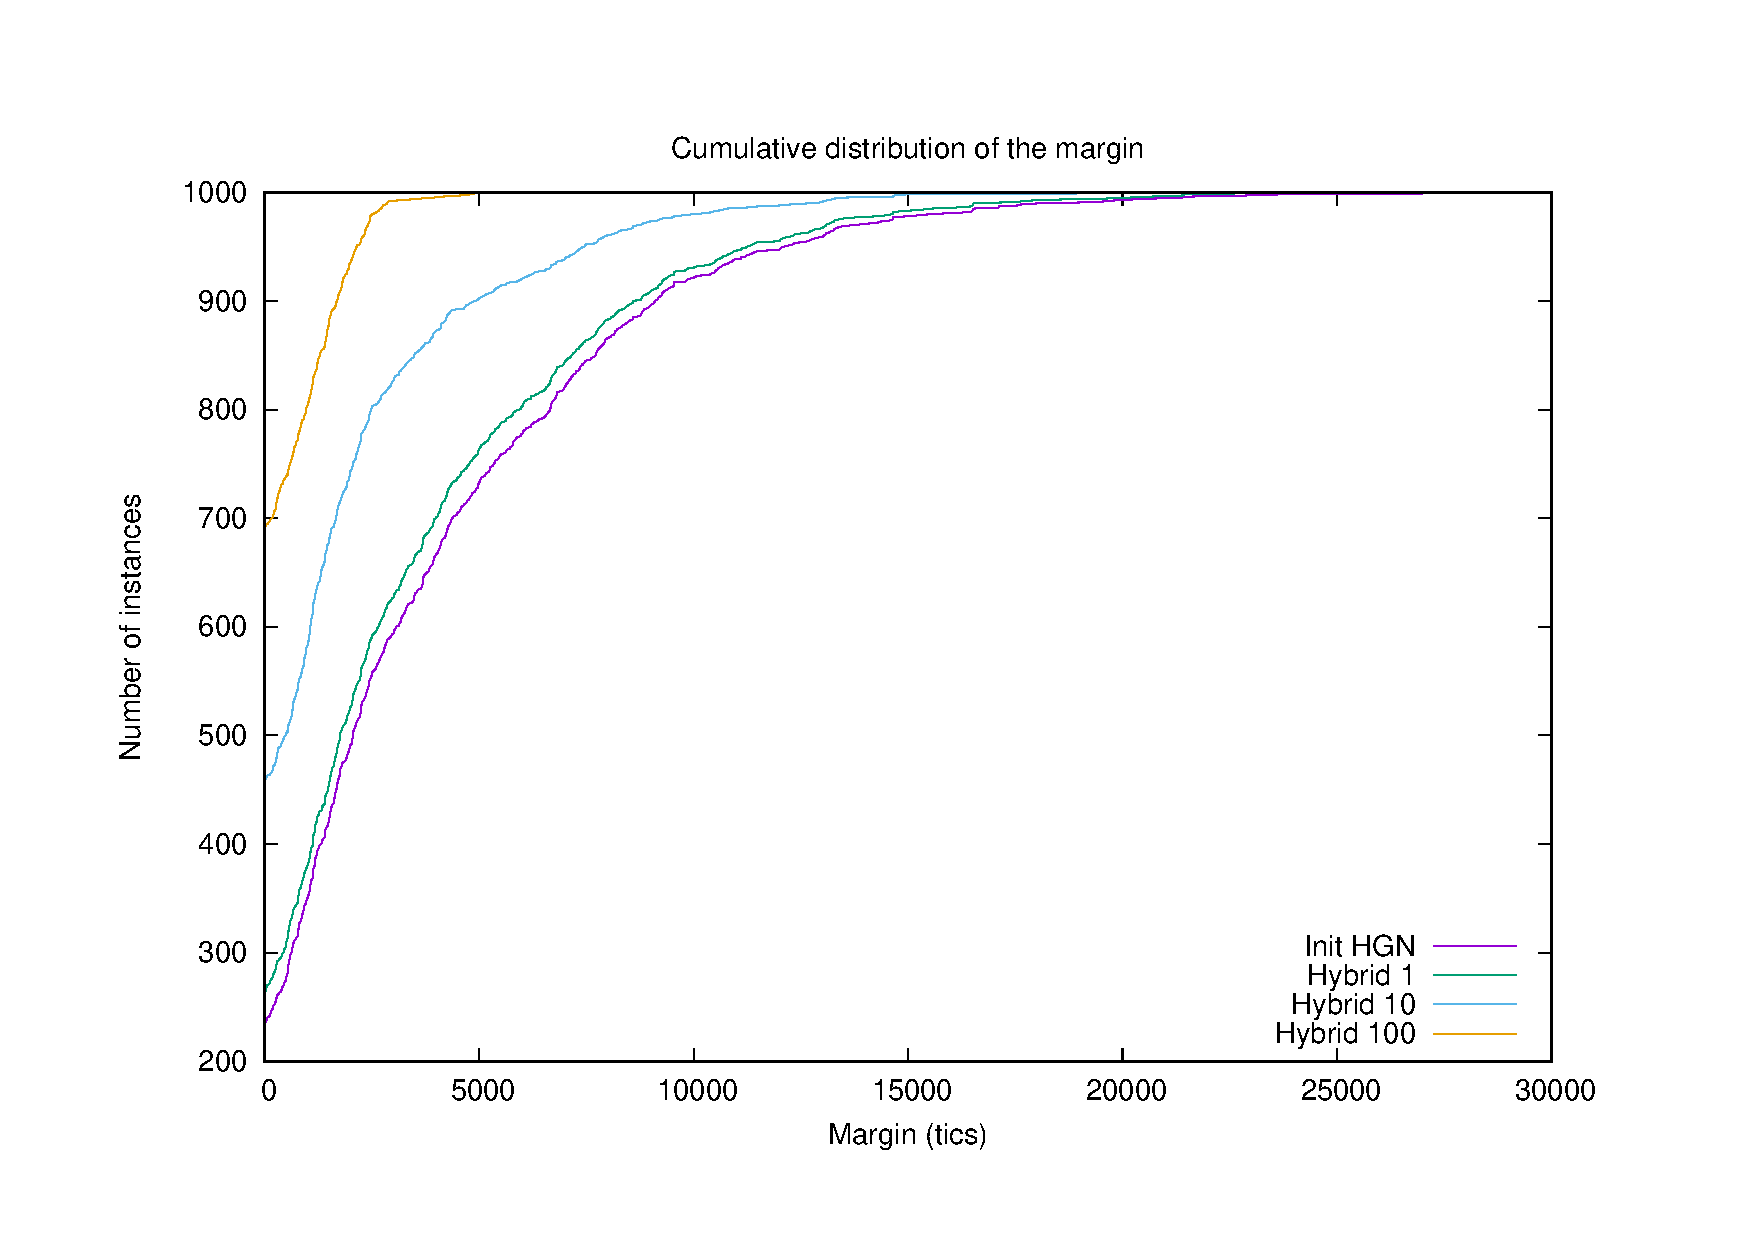
\includegraphics[scale=0.3]{Chapitre5/hybridhill}
\caption{ Margin needed to find a solution for Hill Climbing, intialized with \hgn, hybrid $1$, hybrid $10$ or hybrid $100$. Only the instance for which a solution is found are represented here.}
\label{fig:hybridhill}
\end{figure}

We now focus on how many steps Hill Climbing does before ending in a local optimum. Tabular~\ref{tab:nbstepdescente} shows the average number of steps done by Hill Climbing, for the initial solution giving the best solution. The results in Table~\ref{tab:nbstepdescente} are taken from the experiment done to produce Figure~\ref{fig:hybridhill}.

\begin{center}
\begin{tabular}{ |c|c|c|c|c| }
\hline
     &Init \hgn& Hybrid $1$& Hybrid $10$& Hybrid $100$\\
    \hline
    Average number of steps Step & $1.16$ & $1.23$& $1.77$&$3.52$ \\

    \hline
 \end{tabular}
  \captionof{figure}{Average number of steps needed by Hill Climbing to reach a local optimum. \label{tab:nbstepdescente}}
\end{center}

 The more steps Hill Climbing does, the more the initial solution is improved. When Hill Climbing starts from the result of \hybridgreedynormalized, it does not improve much the solution. When drawing a large number of random compact assignments, the probability of drawing one that can be improved a lot is better and it turns out that compact assignments improved many times are often the one with the best margin.
 
 The idea of drawing a large number of random compact assignments to initialize Hill Climbing is a naive version of Simulated Annealing. The next two presented meta-heuristics are designed to explore the compact assignments, even if a local optimum is reached. Tabu Search remembers the explored solutions, in order to avoid them, and Simulated Annealing browses the compact assignments with a stochastic approach.

\subsection{Tabu Search}

Tabu Search is a variation on Hill Climbing using memory. We start from a compacta ssignment $CA$ given by \hybridgreedynormalized. Then, at each step, from the current compact assignment $CA$, we select the compact assignment $CA'$ which minimizes $TR(CA')$, even when $TR(CA') < TR(CA)$ is not satisfied. To avoid looping around a local minimum, we keep in memory the last $M$ solutions explored and we forbid to visit them again. This algorithm can still loop on a solution cycle larger than $M$, hence we must fix some integer $N$ and stop the algorithm after $N$ steps.
The parameters $N$ and $M$ must be chosen appropriately to minimize the computation time of Tabu Search, while maximising the quality of the solutions found. 

We first investigate on Figure~\ref{tab:tabumn} the impact of $N$ alone. To do so, we fixe $N = M$ (infinite memory) and we compute  Tabu Search on an instance, with $N = 100$, $500$, $1000$ and $2000$. Those simulations have been made with $8$ routes and a load $0.8$, and results are similar for $20$ routes. It appears that with $N=M$, the more steps Tabu Search computes, the better is the solution. For most instance, Tabu Search finds the optimal solutions in the first steps, however for some instances the solution is improved after a large number of steps, which impacts strongly the average margin. At each step, Tabu Search explores the entire neighborhood of the current compact assignment,
which is of the same size for any compact assignment, hence the computation time is linear in $N$. For $N > 500$, the computation time may not be worth the improvement of the solution, as shown in Figure~\ref{tab:tabumn}.



\begin{center}
\begin{tabular}{ |c|c|c|c|c| }
\hline
    N & $100$&$500$& $1000$& $2000$\\
    \hline
    Average number of step & $6.80$ & $10.75$& $10.75$& $29.36$\\
    \hline
    Number of step max & $89$ & $257$& $257$& $1864$\\

    \hline

     Average margin & $2318$ & $2297$& $2297$& $2295$\\

    \hline
    Computation time (s) & $2.0$ & $10.9$& $27.8$& $81.7$\\

    \hline
 \end{tabular}
  \captionof{figure}{Average number of step needed by Tabu Search to reach a local optimum and average value of the margin of this local optimum with infinite memory. \label{tab:tabumn}}
\end{center}


%Thus, we investigate the average number of steps needed by the Tabu Search to find the assignment it returns. Remember that, to each step, the search explores the entire neighborhood of a solution. The computation of Tabu Search is thus exponential in the contention depth and linear in the number of routes.

%Tabu Search has a memory, it remembers the compact assignment for which it explored the neighborhood for the $x$ last solutions in order to not visit them again. Varying the value of $x$ can improve or worsen the performance of the Tabu Search.

We now study the choice of the parameter $M$. Note that increasing may not necessarily decrease the margin
of the solution found by Tabu search. Indeed, a large value for $M$ could restrict the Tabu Search to some component of the transposition graph while a small value of $M$ may allow loops.

We fix $N = 500$ and we compute Tabu Search with $M$ equals $10$, $50$, $100$, $200$ or $500$.
Figure~\ref{tab:tabumemory} shows the cumulative distribution of the margin needed by Tabu Search with different values for $M$. 

\begin{center}
\begin{tabular}{ |c|c|c|c|c|c| }
\hline
    M & $10$&$50$& $100$& $200$& $500$\\
    \hline
    Average number of steps & $2.54$ & $4.97$& $7.42$& $11.38$ & $11.38$\\
    \hline
    Number of step max & $26$ & $67$& $165$& $165$ & $165$\\
    \hline
     Average margin & $3064$ & $2810$& $2722$& $2510$ & $2510$\\
    \hline
 \end{tabular}
  \captionof{figure}{Average number of steps needed by Tabu Search to reach a local optimum and average value of the margin of this local optimum. \label{tab:tabumemory}}
\end{center}

It seems that the more steps Tabu Search remembers, the smaller is the margin of the assignment.
In more of $60\%$ of the cases, Tabu Search finds its best assignment before $10$ steps. When increasing the memory, the average number of steps needed by Tabu Search to find the best solution increases. Nevertheless, remark that for $M > 100$,
the maximal number of steps to find the best solution is $165$. It seems that the memory size has a very small effect on  hard instances.


\subsection{Simulated Annealing}\label{sec:recuit}



In this section, we use the Simulated Annealing method which works as follow.  An initial {\emph temperature} is set and an initial compact valid assignment $CA$ is computed. At each step, we try to replace the current valid compact assignment $CA$, by $CA'$ drawn uniformly at random in the neighborhood of $CA$. Then, in function of the temperature $t$ and $\Delta$ the difference between $TR(Real(CA))$ and $TR(Real(CA'))$, $CA'$ is either accepeted or rejected. More precisely, 
$CA'$ is accepted with probability $e^{-\frac{\Delta}{t}}$. 
After a given number of steps, the temperature is decreased by multiplying it by some constant less than one. The lower the temperature, the lower the chance to accept a compact assignment that worsen the solution. This algorithm is an answer to the exploration/exploitation paradox: in the beginning of the algorithm the whole solution space is explored but as the temperature decreases, the search becomes more and more local around a good solution.


 When using Simulated Annealing, we need to fix the following parameters: initial solution, initial temperature, number of steps before decreasing the temperature, factor by which the temperature is decreased, number of steps without improvement before ending the process. In order to fix the initial temperature $t_0$, we follow~\cite{osman1997meta}:
 \begin{enumerate}
  \item Initiate 100 disturbances at random; evaluate the average $\bar{\Delta}$ of the corresponding variations $\Delta$
\item Choose an initial rate of acceptance $\tau_0$ of the “degrading perturbations” according to the assumed “quality” of the initial configuration; for example:
\begin{itemize}
 \item “poor” quality: $\tau_0 = 50 \%$ (starting at high temperature)
\item “good” quality: $\tau_0 = 20 \%$ (starting at low temperature)
\end{itemize}
\item Deduce $t_0$ from the relation: $e^{-\frac{\bar{\Delta}}{t_0}} = \tau_0$ 
 \end{enumerate}
 
 Tabular~\ref{tab:poorgood} shows the average margin of the solutions produced by Simulated Annealing when initialized with temperatures computed from the previous routine and the computation time. The initial solution used by Simulated Annealing is the solution given by Hill Climbing initialized by \hybridgreedynormalized. The experiment is made on $100$ random instances.
  We experimentally observed that increasing the initial temperature does not significantly improve the quality of the solution, but does increase the computation time. Hence, we assume from now on that the initial solution given by Hill Climbing can be considered as ``good'' to fix the initial temperature.

\begin{center}
\begin{tabular}{ |c|c|c|c|c| }
\hline
 Quality of initial configuration & Good& Poor\\
    \hline
    $t_0$ & $1788$& $4153$\\
    \hline
    Average margin & $4212$ & $4217$ \\
        \hline
    Computation time (ms) &  $2817$&$4035$ \\
    \hline
    
 \end{tabular}
 \captionof{figure}{Comparison of two initial temperatures, considering the quality of the initial configuration}
     \label{tab:poorgood}
 \end{center}

 
 In Simulated Annealing, the temperature should decrease slowly. At each \textbf{level}, $N$ compact assignments are drawn. At the end of a level, the temperature is decreased by $1\%$ and the algorithm stops if less than $1\%$ of the compact assignments drawn are accepted during two consecutive steps. Hence, drawing too few compact assignments in a level decreases the temperature too fast and reduces the efficiency of Simulated Annealing. However, drawing too much compact assignments during a level increases the computation time of the algorithm, there is tradeoff between time an quality and length of a level should be set carefully.


 When $N$ is low ($N=10$ or $N = 20$), the probability of drawing no compact assignment that will be accepted is high and Simulated annealing stops too fast. To fix this issue, we force Simulated Annealing to continue during $10$ consecutive levels for which less than $1\%$ of the compact assignment are accepted. This increases the computation time for higher values for $N$, eventhough Simulated Annealing does not exhibit the problem for these values. Since the neighborhood of a solution is composed of a large number of solutions of the same value, the acceptance rate is greater than $1\%$ even under low temperatures. Hence, we set a minimal temperature under which Simulated Annealing stops.

  
Figure~\ref{tab:recuitmargin} shows the margin needed by Simulated Annealing with different values of $N$. Those results are computed on $1,000$ random instances, in which the initial temperature is set by the routine of~\cite{osman1997meta} presented before and the load is $0.8$


\begin{center}
\begin{tabular}{ |c|c|c|c|c|c|c|c| }
\hline
    $N$ & $10$& $20$& $50$ &$100$&$200$& $500$& $1000$\\
    \hline
    Average Margin & $656$& $378$& $270$ &$257$ & $255$& $249$& $249$ \\
    \hline
    Computation time (s)& $0.11$& $0.33$& $1.3$ &$2.8$ & $5.9$& $15.2$& $30.1$\\
    \hline
 \end{tabular}
  \captionof{figure}{Average Margin of best solution found by Simulated annealing, with a different number of compact assignments drawn at each level.\label{tab:recuitmargin}}
\end{center}

As expected, the computation time is roughly linear in the number of steps $N$. The higher $N$ is, the better is the average margin of the best solution found. It appears that drawing more than $100$ compact assignments at each level does not significantly improve the solution related to the additional computation time. 

 

\section{Branch and Bound}


\subsection{Bruteforcing Compact Assignments}

Solving \spall, means finding an assignment for which $TR(A)$ is minimal. 
Given an instance of \spall, the local search algorithms presented in the previous sections explore a few compact assignments $CA$ and returns the one which minimize $TR(Real(CA))$.  We begin by providing 
a bruteforce algorithm testing all compact assignments, then we show how we can avoid a large number of the compact assignments using a Branch and Bound algorithm, which allows to solve \spall optimally for small number of routes.

\begin{theorem}\label{theorem:FPT}
For routed networks of fixed contention depth $d$, the problem \spall parametrized by $n$ the number of routes is FPT: it can be solved in time $O(nd(n!2^{n})^{d})$.
\end{theorem}
\begin{proof}
The algorithm to solve \spall is the following: all compact assignments $CA$ are generated, for each of them $TR(Real(CA))$ is computed in time $O(nd)$ by Lemma~\ref{lemma:canonical} and we keep the compact assignment for which this value is minimal.  Because of Lemma~\ref{lemma:prec}, to compute the minimum of $TR(A)$, it is enough 
to compute the minimum of $TR(Real(CA))$.

 Now, we need to evaluate the number of compact assignments. 
On a single contention point $c$ with $s = |\mathcal{R}_c|$ routes going through, there are $s!2^s$ possible restrictions of a compact assignment by counting the number of pairs of set and order over $\mathcal{R}_c$.
On a given contention depth consisting in the vertices $\{c_1,\dots,c_l\}$, with $s_i = |\mathcal{R}_{c_{i}}|$, there are 
$\prod_{1 \leq i\leq l} s_i!2^{s_i}$ compact assignments. On a given contention depth, all routes use at most $1$ vertex, hence $\sum_{1 \leq i\leq l} s_i \leq n$. Since $\prod_{1 \leq i\leq l} s_i! \leq (\sum_{1 \leq i\leq l} s_i)!$, we have $\prod_{1 \leq i\leq l} s_i!2^{s_i} \leq n!2^n$. There are $d$ contention depths, thus we have at most $ (n!2^{n})^{d}$ compact assignments which proves the theorem.
\end{proof}

Note that for the vertices of the largest contention depth, compact assignments can be considered independently, since
they do not interact. Let $\{u_1,\dots,u_l\}$ be the vertices of maximal contention depth, and let $s_1,\dots,s_l$
be their width, then we need only to consider $(n!2^{n})^{d-1}(\sum_{1 \leq i\leq l} s_{i}!2^{s_i})$ compact assignments. This makes a large difference in our target application and the experiments presented in this chapter, since in this context $d$ equals three and the $s_i$'s are pretty balanced.

\subsection{Compact Assignment Tree}

From now on, we denote the contention points by ${\cal C} = \{c_1,\dots, c_m\}$,
and we assume they are indexed by contention depth, that is  if $i < j \leq m$ then  $cd(c_i) \leq cd(c_j)$. 

A \textbf{Partial Compact Assignment} $CA$ is a compact assignment defined on a subset ${\cal C}_i = \{c_1,\ldots,c_i\}$ of ${\cal C}$. For a compact assignment $CA$, we denote by $CA_i$ the restriction of $CA$ to ${\cal C}_i$.
Let $CA$ be a partial compact assignment defined on ${\cal C}_{i-1}$, then $CA[(O,S)]$ is an extension of $CA$ to ${\cal C}_{i}$, defined by $CA[(O,S)](c_i) = (O,S)$.  In this section, we build a compact assignment $CA$ by extending partial compact assignments from $c_1$ to $c_m$.


The bruteforce algorithm of Theorem~\ref{theorem:FPT} can be seen as going through a tree of partial compact assignments,
whose leaves are the compact assignments. We call this tree the \textbf{compact assignment tree}. Each vertex $v$ is labeled by a couple $l(v) = (O,S)$ except the root. There is a bijection between a vertex of the tree and a partial compact assignment, such that a vertex at depth $i$ is a partial assignment defined over $\mathcal{C}_i$.
We define the bijecion recursively: let $v$ be a vertex and $u$ its parent, then if $u$ is mapped to $CA$,
and $v$ is at depth $i$, then $v$ is mapped to $CA[l(v)]$.



\subsection{The Branch and Bound Algorithm}


We now explain how to cut the compact representation tree while exploring it by two different means:
the computation of a lower bound of the transmission time over a subtree, to cut the whole subtree and 
several simple rules which eliminates solutions which are dominated by others or which do not yield a valid assignment.


\paragraph{Lower Bounding the Transmission Time}


Once a partial compact assignment is set, one can discard the nodes of the routed network on which it is defined
and work with a simpler routed network, called a \textbf{Restricted Routed Network}. Let $N$ be a routed network
and $CA$ a partial compact assignment defined over $\{c_1\}$, we define the restricted routed network $N(CA)$ by defining a new set of routes ${\cal R}'$ and a new weigth function $\omega'$ as follows. 


A route $r \in {\cal R}$ going through $c_1$, that is equal to $(s,c_1,c_j,\ldots,t)$,  is replaced by the route $(s,c_j,\ldots,t)$ in ${\cal R}'$ while the routes not going throug $c_1$ stay the same in ${\cal R}'$. We define $\omega'(r,s) = \omega(r,s)+\omega(r,c_1) + A(r,c_1)$ where $A(r,c_1)$ is computed from the function $Real(CA_1)$ over the contention point $c_1$, as explained in Section~\ref{sec:real}. To define a restricted routed network obtained from a partial compact assignment defined over ${\cal C}_i$ and a network $N$, we define recursively $N_j = N_{j-1}(CA\restriction_{\{c_j\}})$, with $N_0 = N$. Remark that $CA\restriction_{\{c_j\}}$ is the restriction of $CA$ to the singleton $\{c_j\}$ which is the first contention point of $N_{j-1}$, which makes $N_{j-1}(CA\restriction_{\{c_j\}})$ well defined.


\begin{figure}
\begin{center}
\scalebox{0.6}{

\begin{tikzpicture}
  \SetGraphUnit{5}
    \tikzset{
  EdgeStyle/.append style = {->} }
   \tikzstyle{VertexStyle}=[shape = circle, draw, minimum size = 30pt]
 
\node (k1) at (15,2.25) {\huge{$N$}};



\node (k4) at (12,4.5) {$t_4$};
\node (k3) at (12,3) {$t_2$};
\node (k2) at (12,1.5) {$t_3$};
\node (k1) at (12,0) {$t_1$};

  \node (s4) at (0,4.5) {$s_4$};
  \node (s3) at (0,3) {$s_3$};
  \node (s2) at (0,1.5) {$s_2$};
  \node (s1) at (0,0) {$s_1$};

   \node (t4) at (8,3.75) {$c_4$};
   \node (t3) at (8,0.75) {$c_3$};
   \node (t2) at (4,3.75) {$c_2$};
   \node (t1) at (4,0.75) {$c_1$};

\path (s1) edge [->] node[anchor=north]{\textcolor{blue}{$2$}}  (t1);
\path (s2) edge [->] node[anchor=north]{\textcolor{green}{$7$}}  (t1);
\path (s3) edge [->] node[anchor=north]{$2$}  (t2);
\path (s4) edge [->] node[anchor=north]{$5$}  (t2);

\path (t1) edge [->] node[anchor=north]{$2$}  (t3);
\path (t2) edge [->] node[above right, pos=0.8]{$8$}  (t3);
\path (t1) edge [->] node[above left, pos=0.2]{$1$}  (t4);
\path (t2) edge [->] node[anchor=north]{$6$}  (t4);

\path (k1) edge [<-] node[anchor=north]{$3$}  (t3);
\path (k2) edge [<-] node[anchor=north]{$1$}  (t3);
\path (k3) edge [<-] node[anchor=north]{$2$}  (t4);
\path (k4) edge [<-] node[anchor=north]{$0$}  (t4);





\end{tikzpicture}
}


$\downarrow$

\scalebox{0.6}{

\begin{tikzpicture}
  \SetGraphUnit{5}
    \tikzset{
  EdgeStyle/.append style = {->} }
   \tikzstyle{VertexStyle}=[shape = circle, draw, minimum size = 30pt]
 


\node (k1) at (15,2.25) {\huge$N(CA)$};

\node (k4) at (12,4.5) {$t_4$};
\node (k3) at (12,3) {$t_2$};
\node (k2) at (12,1.5) {$t_3$};
\node (k1) at (12,0) {$t_1$};

  \node (s4) at (0,4.5) {$s_4$};
  \node (s3) at (0,3) {$s_3$};
  \node (s2) at (3,1.5) {$s_2$};
  \node (s1) at (3,0) {$s_1$};

   \node (t4) at (8,3.75) {$c_4$};
   \node (t3) at (8,0.75) {$c_3$};
   \node (t2) at (4,3.75) {$c_2$};

\path (s1) edge [->] node[anchor=north]{\textcolor{blue}{$2$}+\textcolor{red}{$0$}+$2$}  (t3);
\path (s2) edge [->] node[above left, pos=0.3]{\textcolor{green}{$7$}+\textcolor{red}{$1$}+1}  (t4);
\path (s3) edge [->] node[anchor=north]{$2$}  (t2);
\path (s4) edge [->] node[anchor=north]{$5$}  (t2);


\path (t2) edge [->] node[above right, pos=0.8]{$8$}  (t3);

\path (t2) edge [->] node[anchor=north]{$6$}  (t4);

\path (k1) edge [<-] node[anchor=north]{$3$}  (t3);
\path (k2) edge [<-] node[anchor=north]{$1$}  (t3);
\path (k3) edge [<-] node[anchor=north]{$2$}  (t4);
\path (k4) edge [<-] node[anchor=north]{$0$}  (t4);





\end{tikzpicture}
}

 \caption{A restricted routed network $N(CA)$ obtained from $N$ and the partial compact assignment $CA$, defined over $\{c_1\}$, whith $A(1,c_1) = \textcolor{red}{0}$ and $A(2,c_1) = \textcolor{red}{1}$.}

\label{fig:randomnetworks}
\end{center}
\end{figure}

The restricted routed network represents the problem which is left to solve 
when fixing a partial compact assignment.

\begin{lemma}\label{lemma:restriction}
Let $N$ be a routed network, $CA$ a partial compact assignment of $N$, and $\mathcal{CA}$
the set of compact assignments which are extensions of $CA$. Then, $TR(N(CA)) = \min_{ A \in \mathcal{CA}} TR(Real(A))$.
\end{lemma}
\begin{proof}
Let $\mathcal{C}_i$ be the domain of $CA$, by definition of $\mathcal{CA}$, 
for all $A \in \mathcal{CA}$, $A_i = CA$. Let us define the function $Ext$ from the
compact assignments of $N(CA)$ to $\mathcal{CA}$. The assignment $Ext(CA')$ is 
defined as equal to $CA$ over $\mathcal{C}_i$ and equal to $CA'$ over the other contention points.
The function $Ext$ is a bijection and $TR(CA') = TR(Ext(CA'))$, by construction of the restricted routed network
$N(CA)$, which proves the lemma.
\end{proof}

Let $v$ be a vertex of the compact representation tree representing the partial compact assignment $CA$.
If we want to ignore the subtree rooted at $v$ while exploring the partial compact assignment tree,
we must know a lower bound on the transmission time of the compact assignments in this subtree.
Lemma~\ref{lemma:restriction} shows that it is given by the transmission time of the restricted routed network
$N(CA)$, that is solving \spall on a simpler network. Since this value is still too expensive to compute, we provide a relaxation of the problem of solving \spall over $N(CA)$, which is practical to solve.

\paragraph{Relaxation of \spall}

To lower bound the value of $TR(N)$, we propose to transform a routed network into a network with a single contention point, with a lower transmission time (but as large as possible). The problem \spall over a single contention point is the problem \wta, that we have solved in Chapter~\ref{chap:PALL}, and that we can compute efficiently.

Let $N$ be any network and let $c_j$ be a contention point. Let $N^j$ be the routed network with the
single contention point $c_j$, a set of routes $\mathcal{R}'$ and a weight function $\omega'$ defined as follows. For each route $r$ of $N$ which goes through $c_j$, there is a route $r' = (s_r,c_j,t_r) \in \mathcal{R}'$. We define $\omega'(s_r,c_j) = \lambda(r,c_j)$ and $\omega'(c_j,t_r) =  \lambda(r) - \lambda(r,c_j)$. The network $N^j$ represents all the routes going through $c_j$ and assuming further there are no constraint before $c_j$ and after $c_j$.   
Figure~\ref{fig:relaxednetwork} shows a routed network $N$ relaxed to $N^1$ on $c_1$.

\begin{figure}
\begin{center}
\scalebox{0.6}{

\begin{tikzpicture}
  \SetGraphUnit{5}
    \tikzset{
  EdgeStyle/.append style = {->} }
   \tikzstyle{VertexStyle}=[shape = circle, draw, minimum size = 30pt]
 
\node (k1) at (15,3.75) {\huge{$N$}};



\node (k4) at (12,4.5) {$t_4$};
\node (k3) at (12,3) {$t_2$};
\node (k2) at (12,1.5) {$t_3$};
\node (k1) at (12,0) {$t_1$};

  \node (s4) at (0,4.5) {$s_4$};
  \node (s3) at (0,3) {$s_3$};
  \node (s2) at (0,1.5) {$s_2$};
  \node (s1) at (0,0) {$s_1$};

   \node (t4) at (8,3.75) {$c_4$};
   \node (t3) at (8,0.75) {$c_3$};
   \node (t2) at (4,3.75) {$c_2$};
   \node (t1) at (4,0.75) {$c_1$};

\path (s1) edge [->] node[anchor=north]{$2$}  (t1);
\path (s2) edge [->] node[anchor=north]{$7$}  (t1);
\path (s3) edge [->] node[anchor=north]{$2$}  (t2);
\path (s4) edge [->] node[anchor=north]{$5$}  (t2);

\path (t1) edge [->] node[anchor=north]{$2$}  (t3);
\path (t2) edge [->] node[above right, pos=0.8]{$8$}  (t3);
\path (t1) edge [->] node[above left, pos=0.2]{$1$}  (t4);
\path (t2) edge [->] node[anchor=north]{$6$}  (t4);

\path (k1) edge [<-] node[anchor=north]{$3$}  (t3);
\path (k2) edge [<-] node[anchor=north]{$1$}  (t3);
\path (k3) edge [<-] node[anchor=north]{$2$}  (t4);
\path (k4) edge [<-] node[anchor=north]{$0$}  (t4);





\end{tikzpicture}

}
\vspace{1cm}

\scalebox{0.6}{

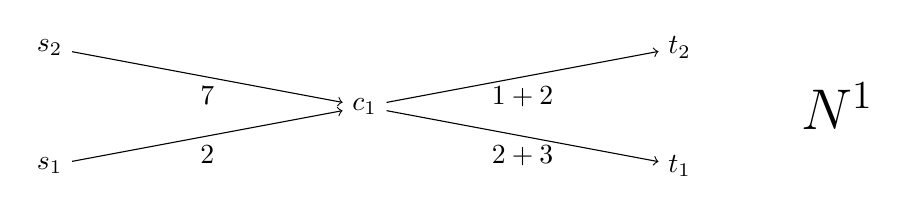
\begin{tikzpicture}
  \SetGraphUnit{5}
    \tikzset{
  EdgeStyle/.append style = {->} }
   \tikzstyle{VertexStyle}=[shape = circle, draw, minimum size = 30pt]

\node (k1) at (14,6.75) {\huge{$N^1$}};
\node (t4) at (12,7.5) {$t_2$};
\node (t2) at (12,6) {$t_1$};
\node (s4) at (4,7.5) {$s_2$};
\node (s2) at (4,6) {$s_1$};
\node (c4) at (8,6.75) {$c_1$};
\path (s2) edge [->] node[anchor=north]{$2$}  (c4);
\path (s4) edge [->] node[anchor=north]{$7$}  (c4);
\path (c4) edge [->] node[anchor=north]{$1+2$}  (t4);
\path (c4) edge [->] node[anchor=north]{$2+3$}  (t2);




\end{tikzpicture}
}
 \caption{Problem \spall relaxed to one contention point.}

\label{fig:relaxednetwork}
\end{center}
\end{figure}


\begin{lemma}\label{lemma:lowerbound}
Let $N$ be a routed network and $c_j$ one of its contention point, then $TR(N) \geq TR(N^j)$.
\end{lemma}
\begin{proof}
We associate to any valid assignment $A$ of $N$, the assignment $f(A)$ of $N^j$
which is defined as $f(A)(r,c_j) = s(r,c_j) - \lambda(r,c_j)$, that is the sum of waiting times in $c_j$ and in contention nodes before $c_j$. By construction of $N$, the transmission time of a route $r$ using $A$ in $N$ is larger than 
the transmission time of the route $r$ using $f(A)$ in $N^j$, since all the waiting times are the same up to 
$c_j$ and they are $0$ for the contention nodes following $c_j$. Hence, we have for all assignments $A$ of $N$,
$TR(A) \geq TR(f(A))$ which proves the lemma. 
\end{proof}


Figure~\ref{fig:relaxednetworkwithass} illustrates Lemma~\ref{lemma:lowervound}. From the routed network $N$ of Figure~\ref{fig:relaxednetwork}, we compute the optimal transmission time of $N^4$. Thus, $A(4,c_4) =$ \textcolor{blue}{$2$} and $TR(N^4) = 13$.
We give in the tabular $A$ the optimal solution for $N$. By considering $A$ and thus $f(A)$, $TR(N^4) = 14$, which is higher than the optimal solution for $N^4$ when solved alone. Remark that, on $N^3$ both solutions are equivalent.




\begin{figure}
\begin{center}

  

\begin{tabular}{ |c|c|c|c|c| }

    \multicolumn{5}{c}{$A(i,c_j)$}\\
    \hline
     $i$ & $c_1$ & $c_2$ & $c_3$ & $c_4$ \\
      \cline{1-5}
    1 & $\textcolor{green}{0}$ & - & $\textcolor{green}{0}$ & -\\
     \cline{1-5}
    2 & \textcolor{red}{$1$}& - & - & \textcolor{red}{$0$} \\
     \cline{1-5}
    3 & - & $\textcolor{orange}{0}$ & $\textcolor{orange}{0}$ & - \\
     \cline{1-5}
    4 & - & \textcolor{blue}{$2$} & - & \textcolor{blue}{$1$} \\
     \cline{1-5}

    \hline
 \end{tabular}

\vspace{1cm}

\scalebox{0.6}{

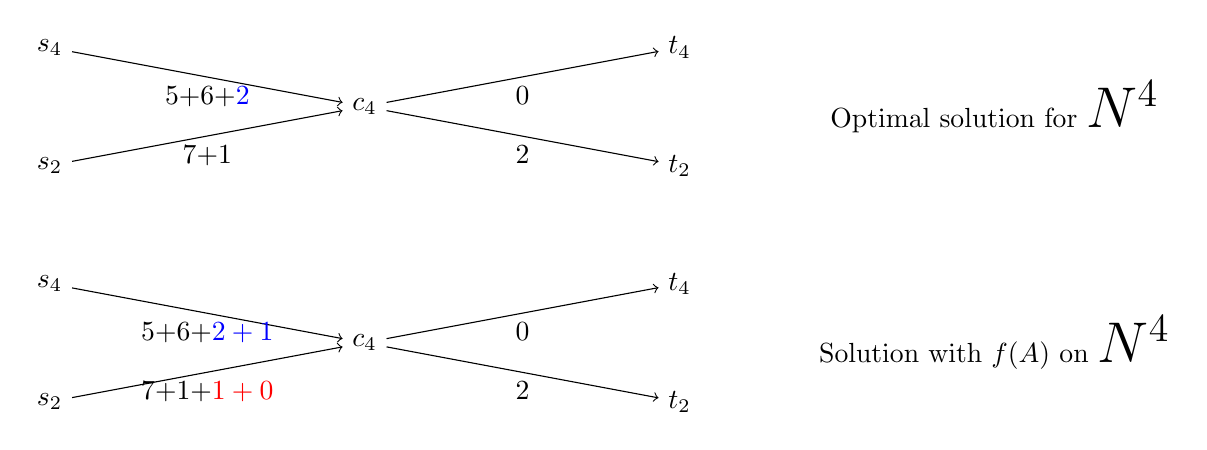
\begin{tikzpicture}
  \SetGraphUnit{5}
    \tikzset{
  EdgeStyle/.append style = {->} }
   \tikzstyle{VertexStyle}=[shape = circle, draw, minimum size = 30pt]
 

\node (k1) at (28,3.75) {Solution with $f(A)$ on \huge{$N^4$}};
\node (t4) at (24,4.5) {$t_4$};
\node (t2) at (24,3) {$t_2$};
\node (s4) at (16,4.5) {$s_4$};
\node (s2) at (16,3) {$s_2$};
\node (c4) at (20,3.75) {$c_4$};
\path (s2) edge [->] node[anchor=north]{$7$+$1$+\textcolor{red}{$1+0$}}  (c4);
\path (s4) edge [->] node[anchor=north]{$5$+$6$+\textcolor{blue}{$2+1$}}  (c4);
\path (c4) edge [->] node[anchor=north]{$0$}  (t4);
\path (c4) edge [->] node[anchor=north]{$2$}  (t2);


\node (k1) at (28,6.75) {Optimal solution for \huge{$N^4$}};
\node (t4) at (24,7.5) {$t_4$};
\node (t2) at (24,6) {$t_2$};
\node (s4) at (16,7.5) {$s_4$};
\node (s2) at (16,6) {$s_2$};
\node (c4) at (20,6.75) {$c_4$};
\path (s2) edge [->] node[anchor=north]{$7$+$1$}  (c4);
\path (s4) edge [->] node[anchor=north]{$5$+$6$+\textcolor{blue}{$2$}}  (c4);
\path (c4) edge [->] node[anchor=north]{$0$}  (t4);
\path (c4) edge [->] node[anchor=north]{$2$}  (t2);



\end{tikzpicture}
}
 \caption{A single contention node $N^4$ on which the optimal assignment is better when solved alone than when solved with the optimal assignment $A$ of $N$, the routed network of Figure~\ref{fig:relaxednetwork}} 

\label{fig:relaxednetworkwithass}
\end{center}
\end{figure}



Let $SCB(N)$, for \emph{Single Contention Bound}, be the function which associates to $N$ the integer 
$\max_{j} TR(N^j)$. By Lemma~\ref{lemma:lowerbound}, we have for all $j$, $TR(N) \geq TR(N^j)$, hence $SCB(N)\leq TR(N)$.
We can compute $SCB(N)$ in time $m2^kk^3log(k)$ where $k$ is the contention width of the network and $m$ the number 
of contention nodes. Indeed, for each $j$, solving \spall on $N^j$ is equivalent to solving \wta, which can be done
in time $2^kk^3log(k)$ by \ASPMLS, where $k$ is the number of routes in $N^j$ which is equal to the contention width of $c_j$ in $N$.

\todo{utiliser la figure du dessus comme exemple ?}

\paragraph{Description of the Branch and Bound Algorithm}

We now describe precisely how the proposed branch and bound algorithm works.
It starts by computing a solution using Simulated Annealing, as described in Section~\ref{sec:recuit},
to initialize an upper bound on the transmission time.
Then, it does a depth first traversal of the compact assignment tree. 
When it enters a node $v$, which represents a partial compact assignment $CA$, it computes $SCB(N(CA))$ and
if it is larger or equal to the upper bound, it backtracks, that is it goes back to the parent of $v$ without visiting
the subtree rooted at $v$. 
When the algorithm reaches a leaf representing some compact assignment $CA$, it computes $TR(Real(CA))$ and updates the upper bound. Lemmas~\ref{lemma:restriction} and~\ref{lemma:lowerbound} proves that the leaves which have not been explored correspond to compact assignments with higher transmission time than the one found by the branch and bound algorithm, proving that it solves \spall.


\paragraph{Additional Cuts}

Even with the cuts due to the evaluation of $SCB(N(CA))$, the compact assignment tree  is still too long to traverse. We propose here several additional cuts that improve the computation time of the algorithm. 

Assume we are at vertex $v$ in the compact assignment tree, representing the partial compact assignment $CA$
over $\mathcal{C}_i$. Let $u$ be a child of $v$, it represents $CA[(O,S)]$, some extension of $CA$ to $\mathcal{C}_{i+1}$. Then, $(O,S)$ is a compact assignment for $c_{i+1}$ in $N(CA)$ and we would like it to be \emph{valid}, \emph{canonical} and \emph{minimal} for $\prec$. Indeed, if $(O,S)$ is not valid for $c_{i+1}$, then none of the extensions of $CA[(O,S)]$ will be valid and we can discard the subtree rooted at $u$.
If $(O,S)$ is not a canonical compact assignment, then by Lemma~\ref{lemma:prec}, there is a a compact assignment $(O',S')$ which is smaller for $\prec$. In the same way, if $(O,S)$ is not minimal for $\prec$, then there is a compact assignment $(O',S')$ which is smaller. In both cases, the transmission time of the extensions of $CA[(O,S)]$ will always be larger than the transmission time of the extensions of $CA[(O',S')]$ and again we can discard the subtree rooted at $u$.


The cut consisting in verifying whether $(O,S)$ is a compact assignment for $c_{i+1}$ in $N(CA)$ is simple to
implement in linear time by computing $Real((O,S))$. 

To guarantee that we only consider canonical compact assignments, we must guarantee that the 
buffering of the first route is zero. It is the same as requiring for a compact assignment $(O,S)$, that $r_{O_1}$, the first route in $O$, is not in $S$. Hence, the cut consist just on discarding assignments with $r_{O_1} \in S$.
This allows to compute normalized sending times for all routes, with $r_{O_1}$ as a reference.

We would like to cut any subtree rooted at a non minimal assignment, but we are not yet able to decide whether a compact assignment is minimal in polynomial time. Hence, we propose several easy to compute heuristics to detect when a compact assignment is not minimal. 
The first one is to consider the assignment $(O,S)$ of $N(CA)$ and for each route
$r_i \in S$, we consider $Real((O,S))$ where $r_i$ has been removed. Then, we try to add back $r_i$, without 
satisfying the constraint on its position in the order but with $r_i \notin S$. If we manage to do so, we have found 
a compact assignment $(O',S\setminus \{r_i\}) \prec (O,S)$. Indeed, routes in $S$ have by definition their sending time
larger than when they are not in $S$ given a fixed first element in the order.
%on pourrait être beaucoup plus précis

For the next cuts, we need to consider that the set $S$ is built incrementally as shown in 
Figure~\ref{fig:partialtree}. We expand a vertex of the compact assignment tree, so that all orders on routes of the contention node are children of the node, then a complete binary tree for each of these orders represents all possible subsets of routes.

\begin{figure}
\begin{center}
\scalebox{0.4}{

\begin{tikzpicture}
  \SetGraphUnit{5}
    \tikzset{
  EdgeStyle/.append style = {->} }
   \tikzstyle{VertexStyle}=[shape = circle, draw, minimum size = 50pt]
 
  \Vertex[x=14,y=14, L = {Root}]{r};
  \Vertex[x=10,y=11, L = {\Large $O_{c_1}=(123)$}]{o1};
  \Vertex[x=18,y=11, L = {\Large $O_{c_1}=(132)$}]{o2};
  \Vertex[x=21,y=11, L = {\Large $O_{c_1}=(213)$}]{o3};
  \Vertex[x=24,y=11, L = {\Large $O_{c_1}=(231)$}]{o4};
  \Vertex[x=27,y=11, L = {\Large $O_{c_1}=(321)$}]{o5};
  \Vertex[x=30,y=11, L = {\Large $O_{c_1}=(312)$}]{o6};

\SetVertexNoLabel
%level 1
  \Vertex[x=5,y=7 ]{s1};
    \node[left] at (s1.south west) {\Large $S_{C_1} = \{\emptyset\}$};
  \Vertex[x=15,y=7]{s2};
  \node[left] at (s2.south west) {\Large $S_{C_1} = \{1\}$};
%level2
  \Vertex[x=2.5,y=4 ]{s3};
    \node[left] at (s3.south west) {\Large $S_{C_1} = \{\emptyset\}$};
  \Vertex[x=7.5,y=4]{s4};
  \node[left] at (s4.south west) {\Large $S_{C_1} = \{2\}$};

  \Vertex[x=12.5,y=4 ]{s5};
    \node[left] at (s5.south west) {\Large $S_{C_1} = \{1\}$};
  \Vertex[x=17.6,y=4]{s6};
  \node[left] at (s6.south west) {\Large $S_{C_1} = \{1,2\}$};
%level 3
  \Vertex[x=0,y=1 ]{s7};
    \node[left] at (s7.south west) {\Large $S_{C_1} = \{\emptyset\}$};
  
  \Vertex[x=20,y=1]{s8};
  \node[left] at (s8.south west) {\Large $S_{C_1} = \{1,2,3\}$};

  \path (s7) edge[dashed] (s8);
  \path (20,7) edge[dashed] (28,7);
  \path (22,4) edge[dashed] (28,4);
  \path (24,1) edge[dashed] (28,1);
  \tikzset{myptr/.style={decoration={markings,mark=at position 1 with %
    {\arrow[scale=3,>=stealth]{>}}},postaction={decorate}}}

    \draw [myptr] (r) -- (o1.north);
    \draw [myptr] (r) -- (o2.north);
    \draw [myptr] (r) -- (o3.north);
    \draw [myptr] (r) -- (o4.north);
    \draw [myptr] (r) -- (o5.north);
    \draw [myptr] (r) -- (o6.north);

    \draw [myptr] (o1) -- (s1);
    \draw [myptr] (o1) -- (s2);
    \draw [myptr] (s1) -- (s3);
    \draw [myptr] (s1) -- (s4);
    \draw [myptr] (s2) -- (s5);
    \draw [myptr] (s2) -- (s6);
    \draw [myptr] (s3) -- (s7);
    \draw [myptr] (s6) -- (s8);
 
%\path (s1) edge [->] node[anchor=south,inner sep = 0.2cm]{$5$} (c1);



\end{tikzpicture}
}
\caption{Expansion of a vertex of the compact assignment tree, corresponding to a contention vertex of width $3$.}

\label{fig:partialtree}
\end{center}
\end{figure}

\begin{itemize}
  \item 
  Assume we are traversing the expansion of a vertex corresponding to the contention vertex $c$.
  In the binary tree, a vertex has two children of depth $i$ representing the fact
  that $r_{O_i} \notin S$ and $r_{O_i} \in S$. We build the partial assignment over $r_{O_1},\dots,r_{O_i}$
  and its realization for $r_{O_i} \notin S$. If $ns(r_{O_1},r_{O_{i-1},c} + \tau = ns(r_{O_1},r_{O_{i},c}$, then
  the two datagrams of the routes $r_{O_{i-1}}$ and $r_{O_{i}}$ follow one another without gap in the period.
  Hence, if we fix $r_{O_i} \in S$, it will not change $ns(r_{O_1},r_{O_{i},c}$ and any extension of this compact assignment will dominated by the extenion of the same compact assignment with $r_{O_i} \notin S$.
  Thus, we cut the branch $r_{O_i} \in S$.

  \item When considering a route $r_{O_i}$ (with $r_{O_i} \notin S$ or $r_{O_i} \in S$), we consider
  the realization of the partial assignments over the elements $r_{O_1},\dots,r_{O_{i-1}}$. If it is possible
  to fix the normalized sending time of $r_{O_i}$ before the normalized sending time of $r_{O_{i-1}}$, without collision,
  then there is a compact assigment $(O',S) \prec (O,S)$ (with $O_i$ at a new, smaller position in O'). It corresponds to
  a compact assignment, with a gap in the period which can be used by some route which should be placed after the gap because of the order. This cut can be computed in linear time, by comparison of the normalized sending times.

  \item To ensure that we go through only canonical assignment, we force the first route $r_{O_1}$ to 
  have zero buffering time, by setting $r_{O_1} \notin S$. But there can be several datagrams with zero 
  buffering time and we refine the notion of canonicity by requiring that the one of smallest id is the
  first in the order. Hence, when we consider $O_i$ with $O_i \notin S$ and that in $Real((O,S))$, 
  $O_i$ as no buffering, then $O_i > O_1$ otherwise we cut the subtree from $O_i \notin S$.
\end{itemize}

\todo{yann: faire une figure qui montre ces trois coupes là (en représentant les paquets avec leur normalized sending time  sur la période)}




\subsection{Scalability with the number of routes}

The complexity of the Branch and Bound algorithm depends on both the contention depth of the routed network and the number of routes. We focus on networks of contention depth $3$, which is realistic in our C-RAN context, and we want to investigate how much the computation time increases in practice when the number of routes grows. Note that the running time
of the algorithm is also very sensitive the width of the network: for the same number of routes, if the routes are well spread out over the contention nodes, there are less compact assignment than if they are concentrated on some contention vertices. In previous experiments, the maximal width is $4$ in the vertices of depth $2$, as shown in Figure~\ref{fig:randomnetworks}. We generalize the topology of Figure~\ref{fig:randomnetworks} by considering any number of 
contention vertex at depth $1$ instead of $4$. Each of theses vertex is of width $2$ and the $2$ routes going through a vertex of depth $1$ are distinct from the other routes and goes to the two different vertices of depth $2$. 

\todo{Yann: mettre un tableau pour dire ce qui vient après et conclure que sans amélioration sur les coupes et l'implémentation on ne peut pas faire $14$ routes (je dirai qu'avec une bonne implèm avec mes coupes plus strictes ou carrément les solutions minimales on devrait atteindre $16$ routes, mais pas mieux)}

Computing an instance with $8$ routes on the network and contention width $4$ takes in average $2,2$s, while it takes $22$s in average for $10$ routes and contention width $5$. Whith $12$ routes and contention width $6$, the computation time increases to $47$ minutes for an instance, on average. Those results are computed on $100$ random instance, with load $0.8$.


\section{Experimental Evaluation}
\label{sec:evalperfspall}
In this section, we compare the performance of all algorithms presented in this chapter.

 We use the settings described in Section~\ref{sec:generationrouted}: There are $8$ routes in the routed network, the length of the arcs are drawn uniformly in $[P]$, and the load is $0.8$.
 The algorithm compared here are:
 \begin{itemize}
  \item \hybridgreedynormalized.
  \item Hill climbing initialized by \hgn.
  \item Hybrid Hill climbing, initialized by $100$ random compact assignments and \hgn.
  \item Tabu Search, with infinite memory and $500$ steps.
  \item Simulated Annealing using $100$ steps by level.
  \item Branch and Bound
\end{itemize}

Figure~\ref{fig:all8routes} shows the cumulative distribution of the margin of the solution found by each algorithm. Tabular~\ref{tab:time8routes} shows the average computation times and margin of the algorithms for the same experiment. The experiment is made on $1000$ instances.

\begin{center}

\begin{figure}[h]
  \centering
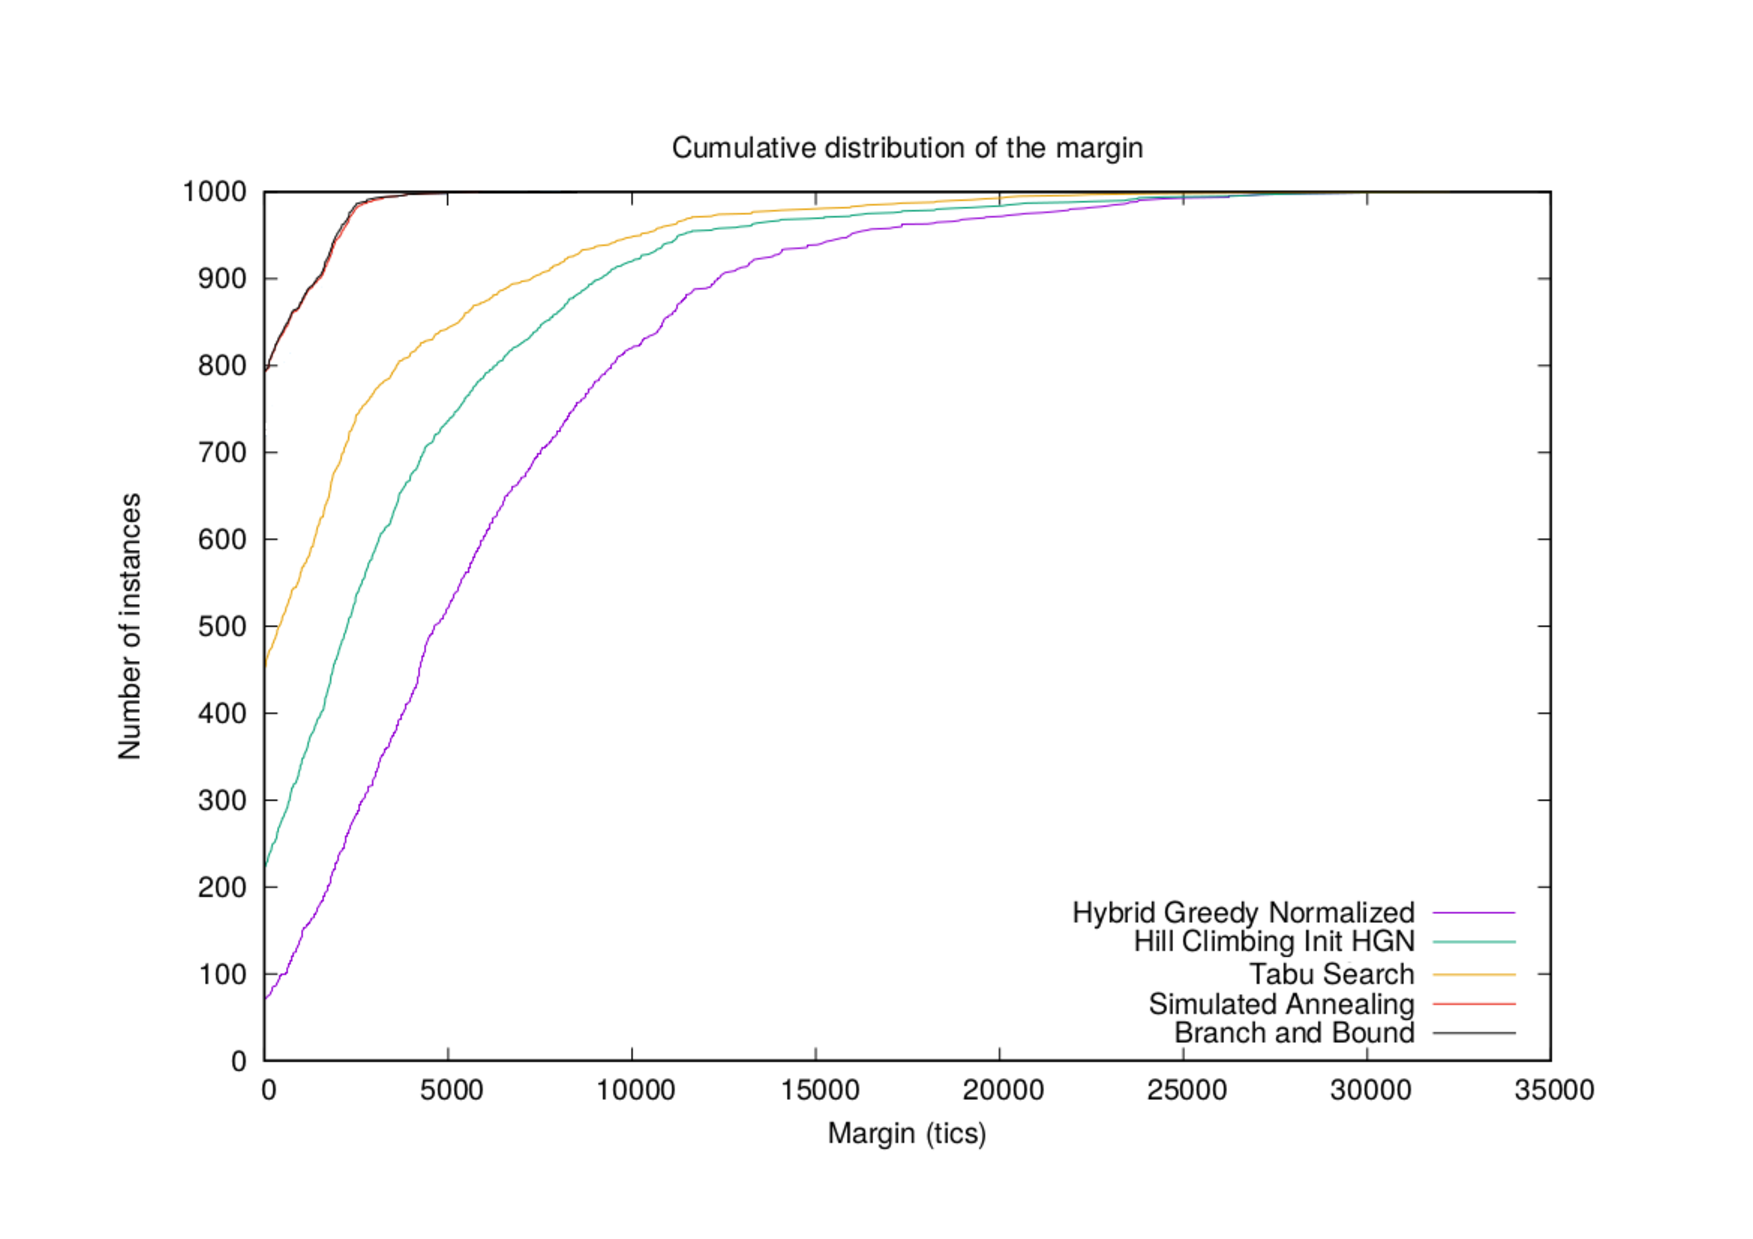
\includegraphics[scale=0.4]{Chapitre5/all8routes}
\caption{ Cumulative distribution of the margin for $8$ routes, length of arcs drawn in $[P]$.}
\label{fig:all8routes}
\end{figure}


\begin{tabular}{ |c|c|c|c|c|c|c| }
\hline
    \tiny{Algorithm} & \tiny{\hgn}& \tiny{Hill Climbing}& \tiny{Hybrid Hill Climbing }&\tiny{Tabu Search}&\tiny{Simulated Annealing}& \tiny{Branch and Bound}\\
    \hline
    \tiny{Margin (tics)} & $5968$& $3666$& $372$ &$2240$ & $294$& $284$ \\
    \hline
   \tiny{Computation time (s)}& $0.005$& $0.035$& $1.39$ &$10.76$ & $2.28$& $0.22$\\


    \hline
 \end{tabular}
  \captionof{figure}{Average margin and average computation time of each algorithm for $8$ routes, length of arcs drawn in $[P]$.\label{tab:time8routes}}
\end{center}

First, remark that \hybridgreedynormalized is far from finding an optimal solution, even when it is followed 
by a Hill Climbing algorithm even though the improvement is important. 
However, computing Hybrid Hill Climbing from $100$ random compact assignments yields solutions which are very close to
the optimal. In these simple settings, it seems to be enough almost explore the whole compact assignment space.
As expected, Tabu Search is better than Hill Climbing computed from the solution of \hybridgreedynormalized, but since it is extremely slow to compute a solution, it is not possible to use it on $100$ different random compact assignments. 
Simulated Annealing is able to compute a good solution, very close to the optimal in the fifth of the time needed by Tabu Search. Branch and Bound is far better than the other algorithms: not only it finds the optimal solution, but it computation time, in this networks with few routes and a small contention width is it $10$ times smaller than Simulated Annealing, while it finds the global optimum.

We now want to compare the performance of those algorithms when the routes are drawn in a small range of values. Thus, we set the length of the routes to be drawn in $[0.9P,P]$. We do the same experiment as previously, but from now on, simulated annealing computes $1000$ compact assignment at each level. As we observed in section~\ref{sec:recuit}, increasing the number of compact assignment considered at each level increases the quality of the solution. While drawing $100$ compact assignments was enough for the simple routed network of the previous experiment,
drawing $1000$ random compact assignments at each level in the two following experiments improves dramatically the performances of Simulated Annealing, with a lower computation time than tabu search.

Figure~\ref{fig:8routessamerange} shows the cumulative distribution of the margin of the algorithms, while Tabular~\ref{tab:8routessamerange} shows the average margin and the computation time of each algorithms on $1000$ random instances.
\begin{center}

\begin{figure}[h]
  \centering
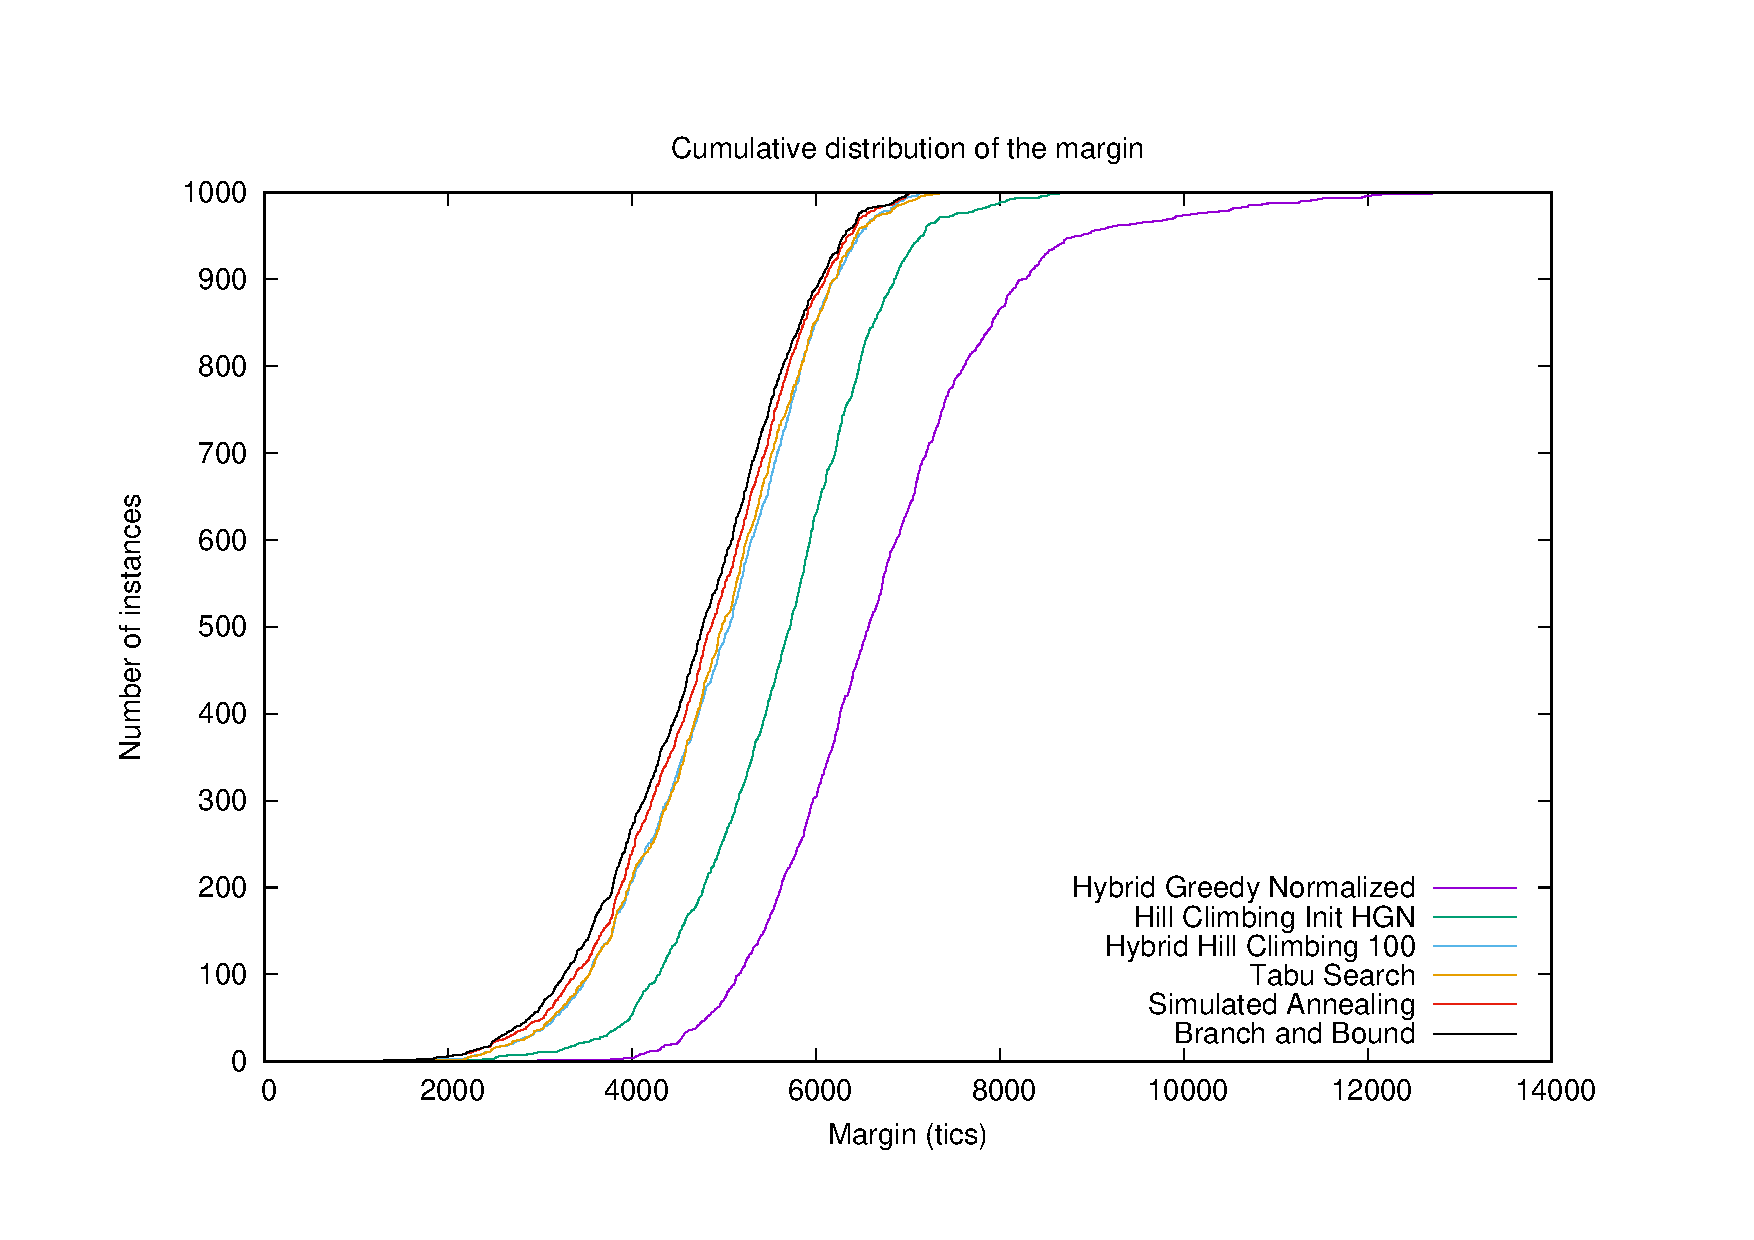
\includegraphics[scale=0.4]{Chapitre5/8routessamerange}
\caption{ Cumulative distribution of the margin for $8$ routes, length of arcs drawn in $[0.9P,P]$.}
\label{fig:8routessamerange}
\end{figure}


\begin{tabular}{ |c|c|c|c|c|c|c| }
\hline
    \tiny{Algorithm} & \tiny{\hgn}& \tiny{Hill Climbing}& \tiny{Hybrid Hill Climbing }&\tiny{Tabu Search}&\tiny{Simulated Annealing}& \tiny{Branch and Bound}\\
    \hline
    \tiny{Margin (tics)} & $6700$& $5636$& $4933$ &$4914$ & $4789$& $4703$ \\
    \hline
   \tiny{Computation time (s)}& $0.004$& $0.048$& $0.965$ &$10.71$ & $6.60$& $0.104$\\


    \hline
 \end{tabular}
  \captionof{figure}{ Average margin and average computation time of each algorithm for $8$ routes drawn in $[0.9.P,P]$.\label{tab:time8routessamerange}}
\end{center}

  We observe that the relative performance of the algorithm does not change. Instances where the length of the routes are drawn in the same range of value needs more margin to be solved. We made the same observation in Chapters~\ref{chap:PAZL,chap:PALL} for different networks and constraints on the assignments.


The following experiment shows the performance of the algorithms when increasing the number of routes. In the instance generated, there are $24$ routes. To do so, we replace each route of the routed network of Figure~\ref{fig:randomnetworks} by three distinct routes. 

This number of routes is too large to compute Branch and Bound. Thus, we also represent $SCB$ in the graph, the lower bound on $TR(N)$ introduced to design the branch and bound algorithm. Figure~\ref{fig:24routes} and Tabular~\ref{tab:24routes} show respectively the cumulative distribution of the margin of the algorithms and the average margin and computation times for the same experiment. The results are computed on $1000$ instance, in which the length of the arcs are drawn in $[P]$.
\begin{center}

\begin{figure}[h]
  \centering
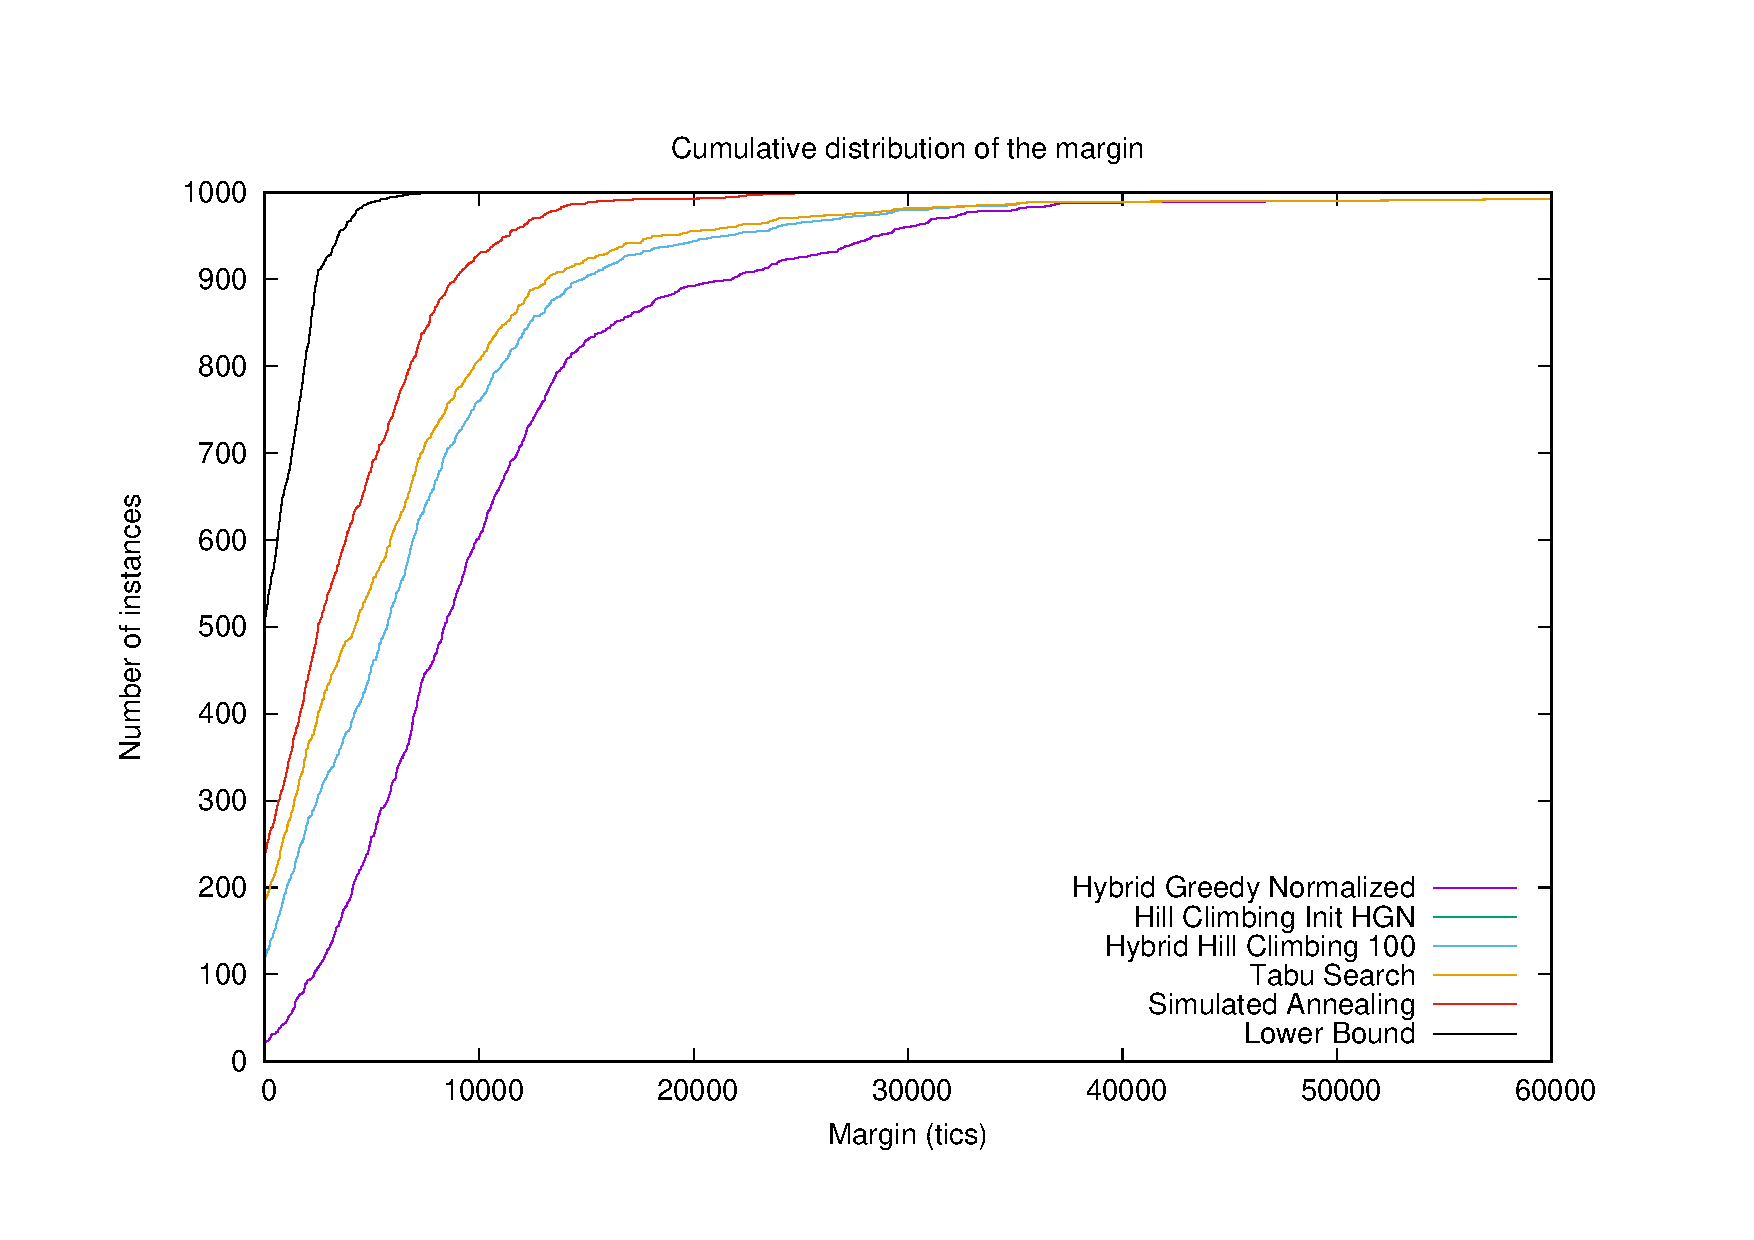
\includegraphics[scale=0.4]{Chapitre5/24routes}
\caption{ Cumulative distribution of the margin for $24$ routes, length of the arcs drawn in $[P]$.}
\label{fig:24routes}
\end{figure}


\begin{tabular}{ |c|c|c|c|c|c|c| }
\hline
    \tiny{Algorithm} & \tiny{\hgn}& \tiny{Hill Climbing}& \tiny{Hybrid Hill Climbing }&\tiny{Tabu Search}&\tiny{Simulated Annealing}\\
    \hline
    \tiny{Margin (tics)} & $10572$& $7402$& $7402$ &$6311$ & $3725$ \\
    \hline
   \tiny{Computation time (s)}& $0.014$& $0.425$& $3.89$ &$55.67$ & $46.32$\\


    \hline
 \end{tabular}
  \captionof{figure}{ Average margin and average computation time of each algorithm for $24$ routes, length of the arcs drawn in $[P]$.\label{tab:24routes}}
\end{center}


First, remark that Hill Climbing has the same performance when it is initialized with $100$ random compact assignments
and the solution given by \hgn or only the solution given by \hgn. As explained in Section~\ref{sec:hillclimb}, the chances to draw a realizable compact assignment is low when the number of routes is large, and we should draw much more random compact assignment to find one which is realizable. It is not reasonable to do so, since we already have 
Simulated Annealing, which does a random search in the space of all compact assigments in a much smarter way.
While the average margin is higher for $24$ routes, than for $8$ routes, Simulated Annealing is still twice better than Tabu Search, its closest competitor, while requiring less computation time.


\subsection{Performance against Statistical Multiplexing}

We now to compare the performance of our best algorithm with the current way to manage networks: Statistical Multiplexing. We use the same simulator as in Section~\ref{sec:statisticalpall}. As a reminder, we propose two policies to deal with buffer in statistical multiplexing. The first one \FIFO, sends the messages in a buffer following the First In First Out policy. The second one, \critdead computes the transmission time of the message in the buffer, if we assume there will not
be buffered anymore, and send the message with the largest transmission time.

We first compare the performances of our best algorithm on $8$ routes: Branch and Bound to statistical multiplexing. Figure~\ref{fig:fptbandb} shows the cumulative distribution of the margin needed by Branch and Bound, and statistical multiplexing using \FIFO or \critdead policy. The experiment has been made on $1000$ instances of load $0.8$, with the lenth of the arcs dranw in $[P]$.

\begin{center}

\begin{figure}[h]
  \centering
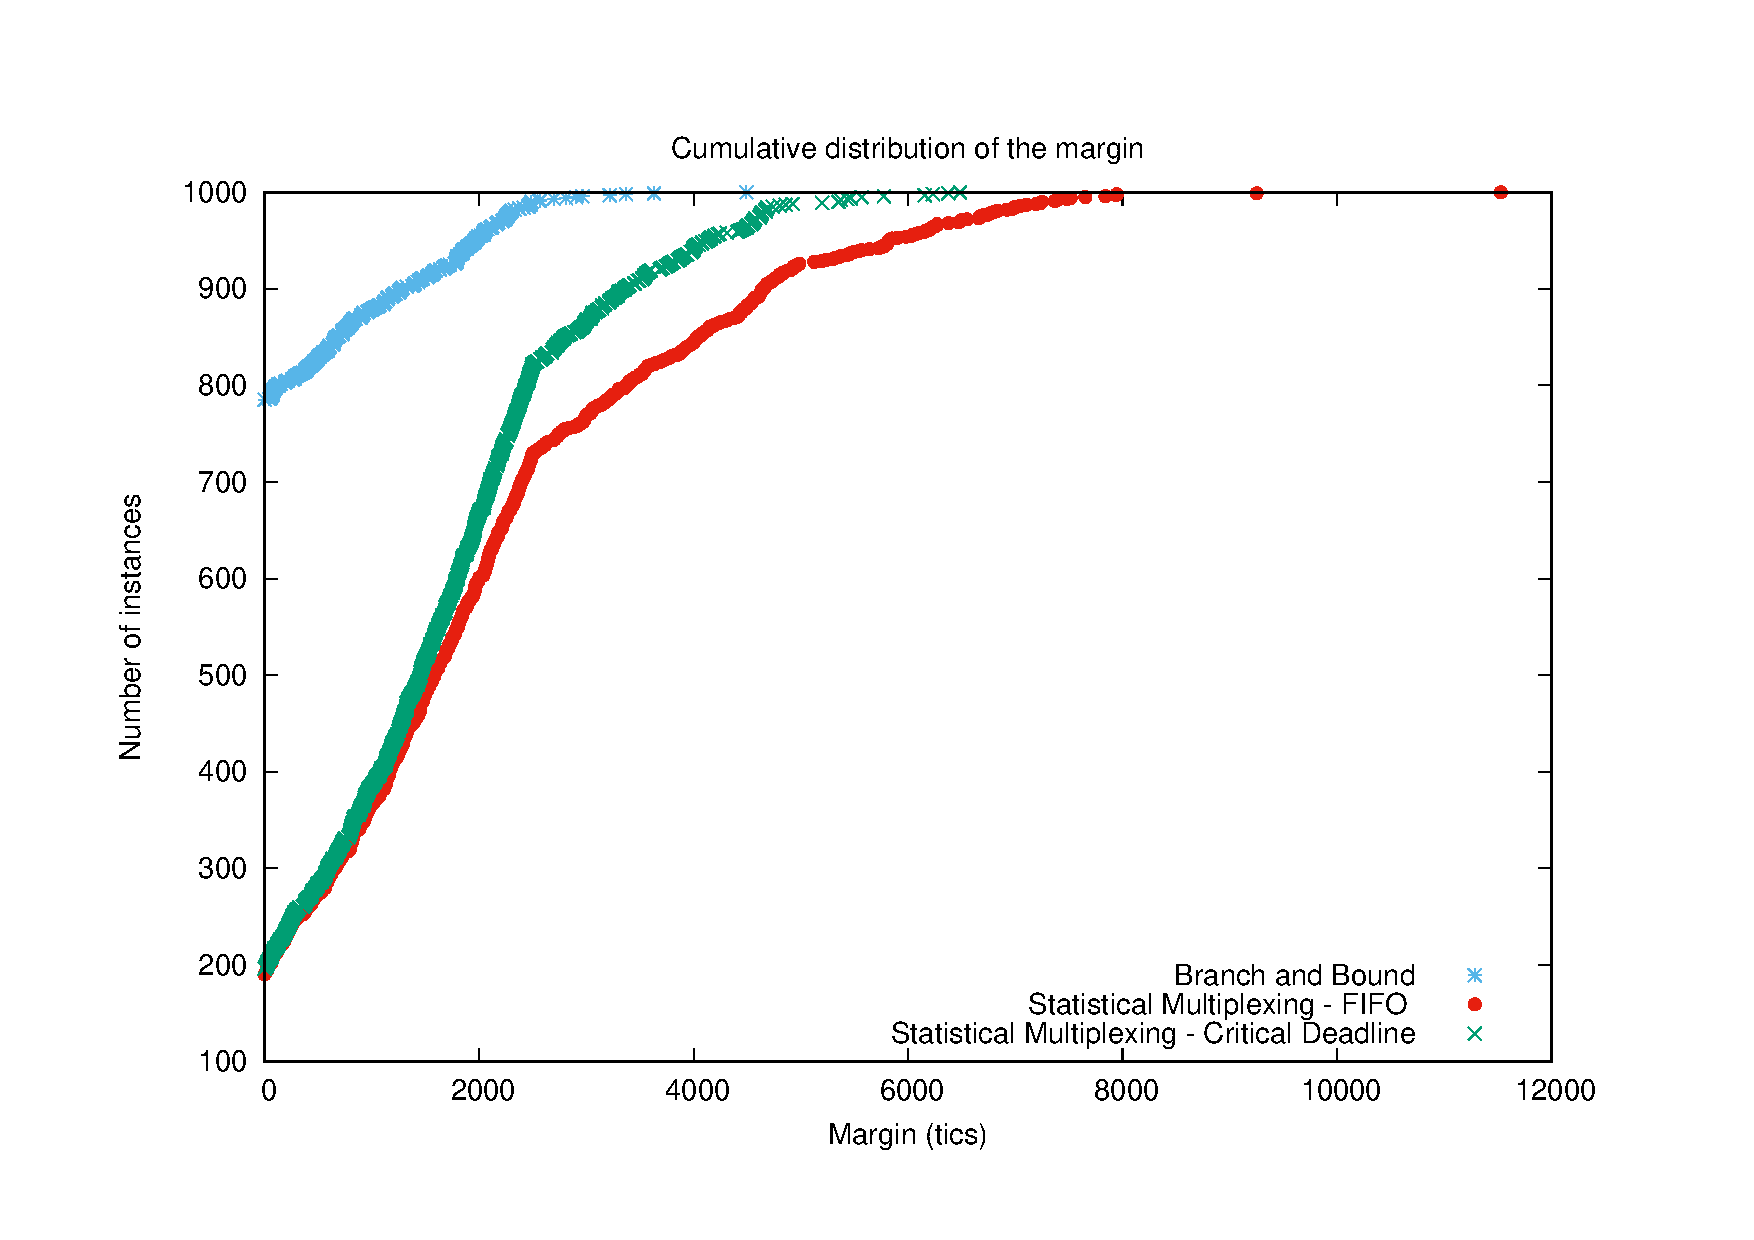
\includegraphics[scale=0.4]{Chapitre5/fptbandb}
\caption{Performance of Banch and Bound Against Statistical Multiplexing for $8$ routes.}
\label{fig:fptbandb}
\end{figure}
\end{center}

Statistical multiplexing using the \critdead policy has a better margin than using \FIFO,
which is expected and similar to Chapter~\ref{chap:PALL}. However, it needs at least $2000$ tics of margin 
to deal with the $80\%$ best instances, while Branch and Bound finds a solution with margin $0$ for its best $80\%$ of the instances.  

We now want to investigate the performance of Simulated Annealing compared to statistical multiplexing when the number of route is too big to execute Branch and Bound.
On Figure~\ref{fig:fptbandb} are represented the cumulative distribution of the margin needed by Simulated Annealing, and statistical multiplexing using \FIFO or \critdead policy. The experiment has been made on $100$ instances of load $0.8$. Here, simulated annealing has been allowed to do $5000$ generation of random compact assignment at each level, because it  increases the quality of the results, with a reasonnable computation time (a few minutes for each instance).


\begin{center}

\begin{figure}[h]
  \centering
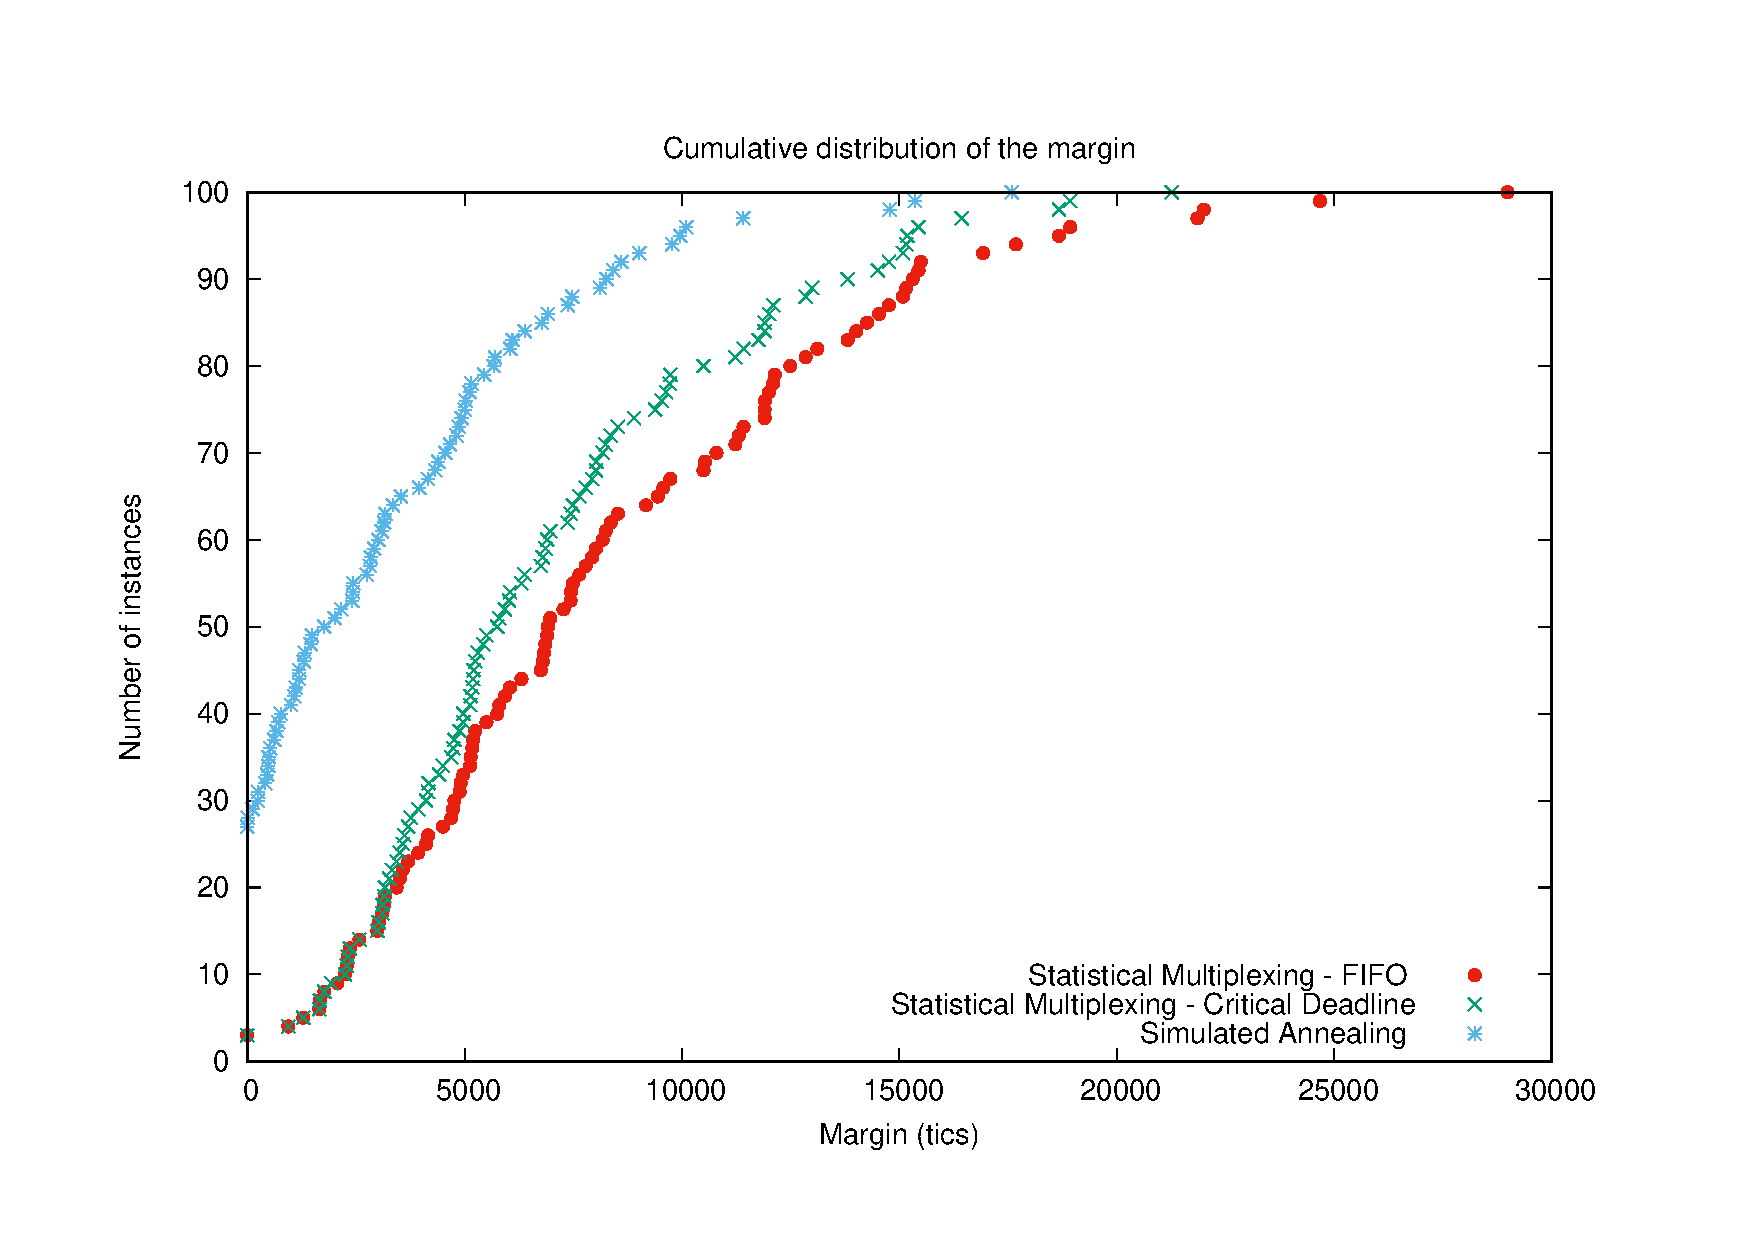
\includegraphics[scale=0.4]{Chapitre5/simanvssto24}
\caption{Performance of Simulated Annealing Against Statistical Multiplexing for $24$ routes.}
\label{fig:simanvssto24}
\end{figure}
\end{center}

Here, the number of instance for which there is an assignment with $0$ margin is lower than in previous experiment, because the instance are harder to solve. Nevertheless, we observe that Simulated Annealing needs about half the margin
of statistical multiplexing using \critdead policy. The average margin is $3329$ for Simulated Annealing, $7516$ for \critdead and $9744$ for \FIFO.



\section{Conclusion}